\documentclass[11pt,letterpaper]{article}
\usepackage[margin=0.88in,headheight=15pt]{geometry}
\usepackage{fontspec}
\setmainfont{TeXGyrePagellaX-Regular.otf}[BoldFont=TeXGyrePagellaX-Bold.otf,ItalicFont=TeXGyrePagellaX-Italic.otf,BoldItalicFont=TeXGyrePagellaX-BoldItalic.otf]
\setsansfont{Liberation Sans}
\setmonofont{DejaVu Sans Mono}[Scale=0.81]
\usepackage{amsmath,amssymb,mathtools,amsthm}
\usepackage{newpxmath}
\usepackage{microtype}
\usepackage{xcolor,graphicx,booktabs,longtable,tabularx,array}
\usepackage{enumitem,fancyhdr,titlesec,needspace}
\usepackage{fvextra}
\usepackage{tikz}
\usetikzlibrary{arrows.meta,positioning,fit,calc}
\usepackage[most]{tcolorbox}
\usepackage{xurl,hyperref,bookmark}
\definecolor{ink}{HTML}{263443}
\definecolor{accent}{HTML}{426452}
\definecolor{pale}{HTML}{F2F5F2}
\definecolor{rulegray}{HTML}{C9D0CC}
\hypersetup{colorlinks=true,linkcolor=ink,citecolor=accent,urlcolor=accent,
 pdftitle={Leant2: A Lean-Native Architecture for Type- and Specification-Directed Synthesis},
 pdfauthor={OpenAI},pdfsubject={Architecture, algorithms, implementation contracts, and checked experiments}}
\urlstyle{same}
\setlength{\parindent}{0pt}
\setlength{\parskip}{5pt plus 1pt}
\setlength{\emergencystretch}{3em}
\setcounter{tocdepth}{2}
\setlist[itemize]{leftmargin=1.5em,itemsep=2pt,topsep=3pt}
\setlist[enumerate]{leftmargin=1.7em,itemsep=3pt,topsep=4pt}
\titleformat{\section}{\Large\sffamily\bfseries\color{ink}}{\thesection}{0.7em}{}
\titleformat{\subsection}{\large\sffamily\bfseries\color{ink}}{\thesubsection}{0.7em}{}
\titleformat{\subsubsection}{\normalsize\sffamily\bfseries\color{accent}}{\thesubsubsection}{0.7em}{}
\pagestyle{fancy}
\fancyhf{}
\fancyhead[L]{\small\sffamily Leant2: architecture and algorithms}
\fancyhead[R]{\small\sffamily September 17, 2026}
\fancyfoot[C]{\thepage}
\renewcommand{\headrulewidth}{0.3pt}
\newcommand{\id}[1]{\texttt{\detokenize{#1}}}
\newcommand{\pathref}[1]{\nolinkurl{#1}}
\newcommand{\Lean}{Lean~4}
\newcommand{\Spec}{\Phi}
\newcommand{\Ctx}{\Gamma}
\newcommand{\Env}{\mathcal E}
\newcommand{\Goals}{\mathcal H}
\newcommand{\Grammar}{\mathcal G}
\newcommand{\sem}[1]{\llbracket #1\rrbracket}
\newcommand{\defeq}{\mathrel{\equiv}}
\newcommand{\pr}{\operatorname{Prop}}
\newcommand{\ty}{\operatorname{Type}}
\newcommand{\sort}{\operatorname{Sort}}
\newcommand{\dom}{\operatorname{dom}}
\newcommand{\FV}{\operatorname{FV}}
\newcommand{\cost}{\operatorname{cost}}
\newcolumntype{Y}{>{\raggedright\arraybackslash}X}
\newcolumntype{L}[1]{>{\raggedright\arraybackslash}p{#1}}
\DefineVerbatimEnvironment{code}{Verbatim}{fontsize=\small,breaklines=true,
 breakanywhere=false,frame=single,rulecolor=\color{rulegray},framesep=5pt,
 commandchars=\\\{\},samepage=false}
% Code is literal; disable commandchars so Lean backslashes are not TeX commands.
\RecustomVerbatimEnvironment{code}{Verbatim}{fontsize=\small,breaklines=true,
 breakanywhere=false,frame=single,rulecolor=\color{rulegray},framesep=5pt,samepage=false}
\newtcolorbox{principle}[1]{enhanced,breakable,colback=pale,colframe=accent,
 boxrule=0.6pt,arc=1mm,title={#1},fonttitle=\sffamily\bfseries,
 left=2mm,right=2mm,top=1.5mm,bottom=1.5mm}
\newtheorem{proposition}{Proposition}[section]
\newtheorem{theorem}[proposition]{Theorem}
\newtheorem{lemma}[proposition]{Lemma}
\theoremstyle{definition}
\newtheorem{definition}[proposition]{Definition}
\theoremstyle{remark}
\newtheorem{remark}[proposition]{Remark}
\begin{document}
\begin{titlepage}
\vspace*{0.45in}
{\sffamily\large\color{accent} TECHNICAL DESIGN STUDY\par}
\vspace{0.3in}
{\sffamily\Huge\bfseries\color{ink} Leant2\par}
\vspace{0.15in}
{\sffamily\LARGE A Lean-Native Architecture for\par Type- and Specification-Directed Synthesis\par}
\vspace{0.4in}
{\large Exact dependent types, joint program/proof search,\par and terminating recursion synthesis\par}
\vspace{0.55in}
\begin{principle}{Central recommendation}
Build an elaboration-aware synthesis engine over exact Lean expressions, not a port of a Haskell type approximation. Its fundamental state should contain a partially constructed program, its dependent typing constraints, and its behavioral proof obligations \emph{together}. Search choices remain revisable until the entire state is solved. Recursion is introduced through typed recursor plans or checked well-founded calls, never by treating the definition under construction as an ordinary available function.
\end{principle}
\vspace{0.3in}
\begin{tabularx}{\textwidth}{@{}L{0.24\textwidth}Y@{}}
Prepared & September 17, 2026 \\
Leant examined & \pathref{6bf05ad78c467989e68290f2d08bbed40802d485} \\
Djex examined & \pathref{e8778f4ebd63e1f9b9b410fa4de8d14a8a04c9e5} \\
Djex pinned by Leant & \pathref{e237e8667190aff38faaa590ce5b12afbffac452} \\
Experimental checker & AXLE, environment \id{lean-4.34.0}; source imports \id{Lean} only \\
Deliverable status & Architecture proposal, small checked Lean prototypes, and a reproducible finite-grammar behavioral experiment; not a complete Leant2 implementation \\
\end{tabularx}
\vfill
{\small Prepared for Vladimir Reshetnikov. Repository observations, proposed mechanisms, and executed experiments are distinguished throughout. No claim about the fraction of practical Lean signatures solved is inferred from the small experimental suite.\par}
\end{titlepage}
\begin{abstract}
Leant2 is designed as a Lean-only successor to Leant and Djex. Native hosting removes a substantial semantic translation boundary, but it does not by itself supply an effective dependent-program synthesis algorithm. The proposed engine combines exact Lean elaboration, dependency-aware bidirectional search, specification propagation, reusable library components, recursion-scheme search, and bounded proof automation. A persistent joint state retains program metavariables, universe constraints, class evidence, residual examples, recursive-call capabilities, and proof obligations under one ownership discipline. This permits a proof failure or a dependent index constraint to revise an earlier program choice rather than merely reject a completed term.

The design specifies search rules, state transactions, candidate indexing, motive generation, counterexample replay, conservative pruning, fair scheduling, memoization, validation, and extension interfaces. It distinguishes finding a typed term, proving its complete specification, refuting one candidate, exhausting a bounded grammar, and proving that the original request has no solution. A small Lean metaprogram checks native dependent search and joint-goal backtracking; a separate indexed-vector experiment checks branch completion inside a supplied recursion skeleton. A finite Python search selects a list-reversal fold, whose universal correctness is then proved in Lean. The experiments also expose two practical boundaries: provisional recursive self-references must be excluded from provider discovery, and indexed case elimination can introduce a standard axiom dependency even when simpler synthesized terms are axiom-free.
\end{abstract}
\tableofcontents
\newpage

\section{What Leant2 should be}
\label{sec:position}

Leant2 should be a \emph{program synthesizer implemented as a Lean elaboration client}, with proof search as one of its cooperating services. It should not be a new type checker, a separate approximation of Lean's type theory, or merely a tactic that tries increasingly many finished expressions and tests them afterward.

The distinction matters for practical requests. A type such as \id{List Nat → List Nat} is easy to inhabit and almost useless as a specification of intended behavior. A type such as a length-indexed vector transformation constrains the output much more strongly, but requires the synthesizer to reason about indices, dependent elimination, and recursion. An additional proposition about a candidate may constrain values, ordering, termination, algebraic laws, or several applications of the function at once. The engine must make useful progress in all three situations without confusing their success criteria.

The proposed architecture has three mutually reinforcing mechanisms. \emph{Type-directed refinement} builds an expression using the exact requested Lean type. \emph{Specification-directed refinement} turns behavioral information into constraints on partially built expressions, supplying counterexamples and pruning only when justified. \emph{Recursion and proof synthesis} select induction structure, recursive motives, and supporting invariants so that common infinite-domain programs need not be discovered as enormous unstructured terms.

\subsection{A practical coverage target, not a fictional completeness target}

The first substantial release should target the following overlapping families: polymorphic higher-order composition; products, sums, structures, and type-class methods; dependent functions and pairs; finite and indexed inductive data; common list, tree, vector, array, and finite-map transformations; arithmetic programs with small decision-procedure obligations; and structurally recursive programs whose invariants can be assembled from available lemmas and bounded templates.

This is a roadmap for \emph{measured coverage}, not a claim that these entire families form one decidable language. Even within a familiar data structure, synthesis difficulty varies enormously. Mapping over a vector is structurally simple. Producing a balanced search tree while preserving ordering, content, and a height invariant requires much stronger construction and proof machinery. A function on natural numbers can encode a difficult theorem in a single refinement.

There should consequently be two complementary modes. A practical, heuristic mode searches an expanding set of useful programs and reports resource-limited uncertainty honestly. Explicit fragment modes fix a grammar, a provider inventory, and a proof discipline; they can support stronger statements about exhaustive exploration of that \emph{specified} search space. Neither mode should infer that a Lean type is uninhabited merely because a search did not find a term.

\subsection{The highest-leverage departures from a literal rewrite}

Native expressions eliminate the need to approximate a dependent family as an opaque Haskell atom, but representation is only the first improvement. The more important algorithmic departures are these:

\begin{enumerate}
\item Keep program and proof holes in one dependency graph. Backtracking must cross the boundary between choosing a witness and proving a property of that witness.
\item Search for a recursion plan and its motive before searching arbitrary recursive syntax. Generalizing an accumulator or an index often changes an intractable search into small constructor and application problems.
\item Propagate exact behavioral information into unfinished code, rather than using behavior only as a completed-candidate filter.
\item Reuse Lean's elaboration and proof-producing facilities while retaining independent candidate validation and explicit operational budgets.
\end{enumerate}

These are engineering commitments with concrete consequences for APIs, caching, scheduling, and tests. The remainder of the article develops them in that order.

\section{What the existing repositories already establish}
\label{sec:baseline}

\subsection{Inspected versions and the limits of this investigation}

The repository review used the revisions on the title page. The Leant submodule entry was read separately: its Djex dependency is \id{e237e8667190aff38faaa590ce5b12afbffac452}, not the later Djex default-branch revision examined alongside it. The review inspected the root documentation, current synthesis and behavioral architecture documents, the earlier Lean rewrite study, and the beginning of the actual fragment translator. It is a targeted architectural investigation, not a complete audit of every module or a rerun of either project's test suites. Source pointers are collected in References~\cite{leant,djex,fragment,behavior,internals,djexarch,rewrite}.

Several existing design decisions are worth preserving. Djinn and Exference are deliberately different search engines. Their shared infrastructure retains type and candidate provenance rather than assuming that pretty-printed text carries adequate semantic evidence. Leant rechecks generated Lean candidates, and its named behavioral assertions are checked by proof attempts about the \emph{exact} proposed candidate. These are stronger foundations than an unchecked Haskell generator followed by example execution.

The recent documentation also records higher-rank, selected polymorphic, dictionary, and universe-aware capabilities. Leant2 should not be motivated by pretending that the current projects only support monomorphic arrows. Their historical test counts are useful regression evidence at their stated revisions, but have not been independently reproduced here and are not used as a current success percentage.

\subsection{The remaining semantic translation boundary}

The inspected \pathref{src/Leant/Synth/Fragment.hs} describes a Lean-side serializer that elaborates a goal and walks its \id{Expr}, then emits an S-expression for a smaller synthesis language. It decomposes supported logical and data structure shapes, preserves selected application and context information, and treats term-indexed applications conservatively as opaque. Certain non-indexed inductives are expanded into sums of products; recursive families retain bounded constructor descriptions. This is a purposeful fragment boundary, not an accidental parser omission~\cite{fragment}.

A native successor can remove this boundary from the \emph{positive synthesis path}. Its application rule can inspect an actual dependent telescope. Its case rule can use actual inductive metadata. Its unification transaction can preserve the exact universe constraints and local instance values selected by Lean. There is no need to translate a variable-length collection of dependent binders into a Haskell approximation and later reconstruct the lost information.

However, a smaller grammar still has value for specialized search. For example, a propositional solver, a bit-vector solver, and a list-fold synthesizer should each have a compact domain representation. The change is that these become \emph{explicit, checked views of one authoritative Lean problem}, not the universal representation to which every supported Lean request must first be reduced.

\subsection{Behavior is already checked; it must additionally guide construction}

Current named behavioral synthesis distinguishes a checked positive assertion, a checked negation, and an inconclusive attempt. Its finite examples establish the supplied finite proposition, not an unstated universal property. The documented proof attempts include \id{decide} and bounded simplification, and preserve candidate ownership~\cite{behavior}.

Leant2 should retain these evidence categories while moving behavioral reasoning earlier. For a dependent witness, a branch predicate, or a recursion algebra, a specification can often constrain an unfinished component before an entire program has been generated. The existing distinction between failed proof search and a proved counterexample remains essential at this finer granularity.

The current indexing-composition reports give a useful acceptance target: finding isolated fold components does not establish that the original compound request is solved under its original limits. A Leant2 evaluation must preserve that distinction. The experiments in this article do not claim to solve the outstanding original integer-indexing or simultaneous-universe composition requests from those reports.

\subsection{Relation to the earlier rewrite study}

The repository already contains a Lean rewrite feasibility analysis. It identifies exact \id{Expr} values, project-specific workers, and retained validation boundaries as sensible directions~\cite{rewrite}. This article adopts that starting point. Its contribution is the more specific synthesis design: a joint dependent search state, stateful refinement transactions, recursion capabilities, motive enumeration, conservative residual semantics, and the contracts that let these parts cooperate. A literal port of the Haskell search engines remains a possible reference implementation, not the recommended final architecture.

\section{The mathematical and operational contract}
\label{sec:contract}

\subsection{A synthesis request}

Let $\Env$ be a fixed imported Lean environment, and let $\Ctx$ be an ordered local telescope. The telescope includes definitions as well as variables; later declarations may depend on earlier ones. A logical request consists of
\[
 \Env;\Ctx \vdash T : \sort u,
 \qquad
 \Env;\Ctx \vdash \Spec : T \to \pr.
\]
Without an explicit behavioral condition, $\Spec$ is the constant true predicate. A successful result supplies both
\begin{equation}
 \Env;\Ctx\vdash e:T,
 \qquad
 \Env;\Ctx\vdash p:\Spec(e).
 \label{eq:success}
\end{equation}
This is a meta-level pair of artifacts. It need not be encoded as a \id{Sigma}: ordinary \id{Sigma} has restrictions on its sorts, and a proposition-valued second component is not automatically the type of an ordinary dependent pair. For an executable target $T:\ty u$, a Lean subtype is often a convenient certificate-carrying output; the general engine should keep expression and proof fields separately.

The operational request additionally fixes a grammar or grammar policy, a permitted provider inventory, transparency settings, an axiom and execution policy, a ranking policy, and resource limits. These are part of reproducibility. Changing the available providers changes what can be found; changing the axiom policy changes which proofs are acceptable; changing a budget changes what an unsuccessful run establishes.

\subsection{Exact treatment of the surrounding context}

A standalone command should elaborate the requested type and predicate before search, reject unresolved names, and either resolve elaboration metavariables or assign them an explicit ownership category. It must not silently turn a misspelled identifier into an additional implicit parameter.

A tactic runs in a more complicated situation: its target may share metavariables with other goals. The default should treat externally owned metavariables as rigid. An advanced integration may grant a query ownership of an explicit set of shared metavariables, but then its result is an atomic assignment patch for the full affected state, not merely a term for one visible goal. No worker may commit a substitution that changes an unrelated elaboration obligation without the owner's approval.

Named universe parameters of a declaration are rigid. Fresh level metavariables used to instantiate a library constant are flexible. This distinction prevents the engine from ``solving'' a universe-polymorphic request by specializing the requested universe to zero. A successful export retains the requested universes and binders, even when the chosen implementation happens not to use all of them.

\subsection{Result categories}

\begin{longtable}{@{}L{0.22\textwidth}L{0.72\textwidth}@{}}
\toprule
Result & Meaning and required evidence \\
\midrule
\endhead
Typed candidate & A checked $e:T$. No unproved behavioral assertion is implied. \\
Specified candidate & The pair in~\eqref{eq:success}, checked against the exact query and admitted dependencies. \\
Finite observations passed & The named observations succeeded. Unless their conjunction is the entire request, this is not a complete-specification result. \\
Candidate refuted & A proof of $\neg\Spec(e)$, or a replayed input that supports such a proof for the specified property. Only this candidate is refuted. \\
Original request refuted & A checked proof of $\neg\exists e:T,\Spec(e)$; without a specification, a checked proof of $\neg\operatorname{Nonempty}(T)$. \\
Grammar exhausted & No accepted solution in a precisely identified finite grammar and checking regime, with its completeness conditions recorded. This does not imply the original request is impossible. \\
Unknown & Budget exhaustion, unsupported reasoning, solver uncertainty, interrupted elaboration, or another explicitly reported incomplete outcome. \\
\bottomrule
\end{longtable}

The query predicate can itself be a finite conjunction of examples. In that case a proof of exactly that conjunction \emph{is} a specified candidate. The distinction is between the proposition actually requested and a stronger proposition inferred by the reader, not between ``examples'' and ``proofs'' as mutually exclusive categories.

\subsection{Executable and logical requests are different products}

A proof of an existential proposition is not always a usable program implementing its witness extraction. Lean's elimination rules distinguish propositions from computational data, and a noncomputable choice of a witness is not an executable algorithm. Leant2 should expose this distinction directly: a request for a runnable function uses an executable policy, while a request for a classical existence proof may permit noncomputable terms.

Similarly, a function returning \id{Option A} is not automatically a terminating program. Its declared result type models failure, but says nothing by itself about whether its compiled implementation terminates. The proposed executable profile allows only admitted total definitions, verified recursion plans, and explicitly approved runtime dependencies. Search code itself may use partial recursion: the termination of the synthesizer and the termination of the synthesized program are separate concerns.

\section{Component architecture and process boundaries}
\label{sec:architecture}

\begin{figure}[htbp]
\centering
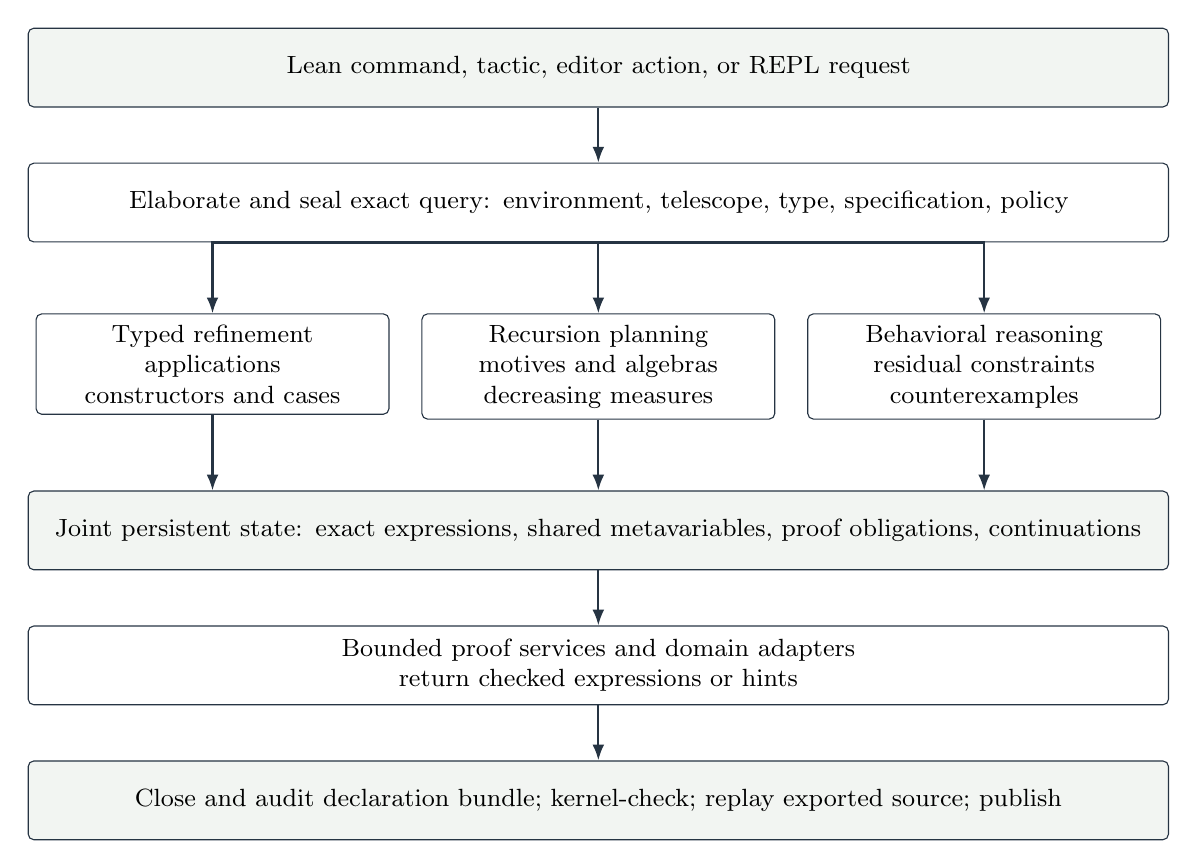
\begin{tikzpicture}[
 box/.style={draw=ink,rounded corners=2pt,align=center,font=\small,
              text width=42mm,minimum height=10mm,inner sep=4pt},
 wide/.style={box,text width=142mm},
 arrow/.style={-{Latex[length=2mm]},thick,draw=ink}]
\node[wide,fill=pale] (front) {Lean command, tactic, editor action, or REPL request};
\node[wide,below=7mm of front] (seal) {Elaborate and seal exact query: environment, telescope, type, specification, policy};
\node[box,below=9mm of seal,xshift=-49mm] (struct) {Typed refinement\\applications\\constructors and cases};
\node[box,below=9mm of seal] (recur) {Recursion planning\\motives and algebras\\decreasing measures};
\node[box,below=9mm of seal,xshift=49mm] (behavior) {Behavioral reasoning\\residual constraints\\counterexamples};
\node[wide,below=9mm of recur,fill=pale] (joint) {Joint persistent state: exact expressions, shared metavariables, proof obligations, continuations};
\node[wide,below=7mm of joint] (proof) {Bounded proof services and domain adapters\\return checked expressions or hints};
\node[wide,below=7mm of proof,fill=pale] (check) {Close and audit declaration bundle; kernel-check; replay exported source; publish};
\draw[arrow] (front)--(seal);
\draw[arrow] (seal.south)-|(struct.north);
\draw[arrow] (seal)--(recur);
\draw[arrow] (seal.south)-|(behavior.north);
\draw[arrow] (struct.south)--(struct.south |- joint.north);
\draw[arrow] (recur)--(joint);
\draw[arrow] (behavior.south)--(behavior.south |- joint.north);
\draw[arrow] (joint)--(proof);
\draw[arrow] (proof)--(check);
\end{tikzpicture}
\caption{One semantic problem and one candidate authority, with several cooperating search services. The boxes above validation are not trusted to establish success merely by returning a status flag.}
\label{fig:architecture}
\end{figure}

\subsection{A library in the project toolchain}

The core package should be a Lean library compiled with the project's own toolchain. A small adapter layer isolates version-sensitive elaboration APIs. The public entry points elaborate syntax and construct a sealed problem; the search engine operates on that problem, not on strings. The result can be inserted into a tactic goal, rendered as a declaration, or returned to a REPL.

The controller may also be written in Lean. For interactive use, it should communicate with a replaceable project-local worker process. This preserves the ability to retire a timed-out or corrupted worker, keeps compiled module versions aligned, and avoids pretending that a serialized in-memory Lean environment is a stable cross-version interchange format. The worker owns its environment, local contexts, and metavariable identifiers.

A standalone implementation does not need a separate service process for every search rule. Fine-grained work stays in the worker; heavyweight solver calls and untrusted runtime evaluations can use subordinate processes. The logical core should work without an external SMT installation. Optional adapters can add solver-assisted proposal and reconstruction without changing the meaning of a successful result.

\subsection{Two representations, with different jobs}

There should be exactly one authoritative representation of Lean terms and types: Lean expressions in an identified environment and scope. A second, small \emph{search-plan representation} describes choices such as ``introduce this binder,'' ``apply this provider with these arguments,'' ``split this discriminant,'' or ``instantiate this recursion plan.'' It stores continuations and provenance; it does not define an alternative typing relation for general Lean.

For persistent logs and process boundaries, expressions are closed over a telescope and associated with their environment identity. Cross-process records use scoped binders and declaration references, not raw \id{FVarId} or \id{MVarId} values. An imported recipe recreates fresh identifiers and is rechecked. A successful candidate may be transmitted as exact source plus an explicit declaration bundle; the new process treats that as input to validation, not as already trusted proof.

Specialized solvers may have their own ASTs. Each such AST has an explicit interpretation into a fragment of the sealed Lean query. The adapter records what is exact, what is an over-approximation, and which statements can return as proofs. This avoids rebuilding the old approximation boundary in a different programming language.

\subsection{Immutable ownership and mutable services}

The query, imported environment snapshot, provider inventory, and completed candidate packages should be immutable. Search nodes may refer to persistent Lean states and shared expression DAGs. The global scheduler, counters, cancellation token, and bounded caches are mutable services, but they must not become additional authorities for the candidate's meaning.

The distinction is particularly important for counterexamples. A counterexample bank belongs to an exact specification and interpretation policy. A sample valid for one instance dictionary, scalar type, or machine-integer semantics must not leak into a superficially similar request with different meanings. Candidates retain their own exact expression and provider selections even when they are placed in the same ranking bucket.

\section{The joint dependent search state}
\label{sec:state}

\subsection{State contents}

A useful abstract state is
\begin{equation}
 S=(Q,\sigma,\Goals,D,R,E,V,K,\rho).
 \label{eq:state}
\end{equation}
Here $Q$ is the sealed query; $\sigma$ is the saved elaboration/metavariable state; $\Goals$ is the set of outstanding holes and constraints; $D$ is their dependency graph; $R$ contains recursive-call capabilities; $E$ is the current observation set and residual semantics; $V$ records speculative choices and their continuations; $K$ is branch-local cost and feature information; and $\rho$ identifies the replay recipe.

A hole records its exact type and local telescope. Its category identifies whether it is a program value, a type argument, an index, a proof, a class instance, a universe assignment, or a recursion motive. Categories guide scheduling, not typing: a natural-number index is still a Lean term, and a class dictionary is still a value whose identity can affect behavior.

A dependency edge $h_1\to h_2$ means that assigning $h_1$ can change the type, admissibility, or specification of $h_2$. This includes occurrence in types and terms, but also deliberately tracked semantic dependencies, such as an example residual whose evaluation is blocked on $h_1$. Recomputing a node need not invalidate every cache: explicit dependency tracking allows precise invalidation.

\subsection{Why independent goal solving loses programs}

Consider a type of certified choices:
\begin{code}
inductive Choice where | first | second
inductive Good : Choice -> Prop where | second : Good Choice.second
-- Target:
{c : Choice // Good c}
\end{code}

A constructor step creates a value hole $?c:\id{Choice}$ and a proof hole $?p:\id{Good}(?c)$. The first type-correct value may be \id{Choice.first}. If the value solver returns this as a final answer and forgets its alternatives, the proof solver cannot repair the result. The correct algorithm retains the value choice point while solving the proof. Failure of \id{Good Choice.first} returns to the choice of $?c$, allowing \id{Choice.second}.

The problem is not restricted to subtypes. A type parameter selected for one application argument can constrain another argument several binders later. An index inferred in a constructor field can determine the type of a later field. A class instance selected at one use can change the behavioral meaning of a method elsewhere. An AND-node is therefore a \emph{joint obligation with correlated substitutions}, not a Cartesian product of independent first answers.

\begin{principle}{Commit criterion}
A subgoal solution may be memoized as an alternative, but its assignments become irrevocable only when all dependent obligations in the enclosing branch have been discharged or the resulting generalization has been independently justified.
\end{principle}

\subsection{Transactions must include failed unification}

Lean's metavariable operations are stateful. A refinement attempt may instantiate several metavariables before discovering a conflict or reaching a limit. Every speculative action must therefore run from a saved state and either publish its complete successor state or restore the original state. A catch block that returns ``failure'' without restoration is not a correct backtracking boundary.

The production transaction should cover the metavariable context, relevant elaboration state, local-instance state, diagnostic state, and any environment extension created by the action. Merely restoring one expression-valued substitution map is insufficient. The safest initial implementation serializes actions over a complete saved state through a small version-specific adapter; optimized deltas can be introduced after equivalence tests exist.

Resource charges must \emph{not} roll back. Failed alternatives consume search time, elaboration heartbeats, memory, and solver work. A separate monotone ledger records that work. Otherwise a branch can repeatedly retry an expensive failing action while appearing never to consume its allowance.

\subsection{Three different meanings of ``blocked''}

A hole may be blocked because its type depends on an unresolved metavariable. It may be blocked because the engine lacks a suitable synthesis rule or domain interpretation. Or it may have exhausted its current local allowance. These cases should produce distinct states:

\begin{code}
blockedOnAssignments(dependencies)
unsupportedByLane(feature, continuation)
yieldedForBudget(continuation, chargedWork)
\end{code}

None is a contradiction. The scheduler can awaken the first after a substitution, route the second to another lane, and resume the third after a fair turn or an explicitly enlarged bound. Replacing all three by an empty list of candidates obscures both completeness accounting and performance diagnosis.

\subsection{Proof search may choose data inadvertently}

A proof goal containing a program metavariable is not purely a proof-search problem. A tactic proving $?x=7$ by reflexivity can assign $?x:=7$. That can be useful specification-directed synthesis, but it must be treated as a branch choice, with full transaction and cost accounting. An ordinary proof service must not silently acquire permission to commit arbitrary code assignments.

There are two sound integration modes. In \emph{joint mode}, the proof service returns its complete assignment patch as a speculative successor. In \emph{proof-only mode}, all computational holes are already fixed, or they are replaced by suitably scoped rigid parameters and the service proves a theorem universally quantified over those parameters. The latter proof is stronger and may be harder, but can be reused for any later filling. Relying on a vaguely ``opaque'' metavariable convention without testing what the selected Lean API actually permits is not enough.

\section{The main search algorithm}
\label{sec:search}

\subsection{A resumable best-first portfolio}

The outer algorithm operates on resumable node actions rather than on opaque calls that must finish producing a candidate before yielding. The following is algorithmic pseudocode, not a claim that these API names already exist:

\begin{code}
solve(query):
    initial := elaborateAndSeal(query)
    frontier := initialStates(initial)
    while budget.remaining and frontier.hasWork:
        (lane, node, action) := scheduler.nextQuantum(frontier)
        charge := beginNonrefundableWork()
        outcome := runTransaction(node.snapshot, action, quantum)
        charge.finish(outcome.work)
        match outcome:
          successors(children): enqueue(children)
          yielded(cursor):      retainContinuation(cursor)
          candidate(term):      validateOrScheduleProof(term)
          checkedPrune(proof):  closeExactBranch(proof)
          failedAttempt(reason):recordLocalFailure(reason)
          interrupted:          stopWithUnknown()
    return resultsWithEvidenceAndTerminationReason()
\end{code}

Each lane is a policy over the same core actions: cheap structural completion, library composition, recursion planning, dependent constraints, or specialized behavioral sketches. Lane identity does not change what a candidate means. Candidate generation, proof validation, and counterexample replay all spend the same query-wide resources, with independently visible subtotals.

A simple prototype can implement the joint-state semantics by recursively searching a list of goals, wrapping the solution of a head goal \emph{and the entire remaining list} in one transaction. The supplied Lean prototype does exactly that. A production engine should retain explicit continuations and persistent states to avoid recomputing large successful prefixes after a later failure.

\subsection{Focused introductions}

When the weak-head-normalized target is a dependent function type, introduce a fresh local with the exact binder information and search the body:
\[
 \frac{\Ctx,x:A\vdash e:B(x)}{\Ctx\vdash \lambda x.e:(x:A)\to B(x)}.
\]
Preserve implicit, strict-implicit, and instance-implicit binders. The search state knows the fresh local's actual identity, not merely its printed name. If a specification is about the function as a whole, retain it; pointwise examples can additionally be projected into the body after substituting their arguments.

Introduction is a useful focusing step because it avoids constructing redundant partially applied combinators. It is not a license to erase every behaviorally distinct alternative. The engine should state which normal forms it searches modulo a justified equality, and preserve source-level variants only as presentation choices. Constructor selection for a sum or a data-valued structure is ordinarily a real choice.

For a structure or an inductive target, create a constructor application through Lean's actual constructor type. Instantiate parameters and indices, create dependent field holes in telescope order, and keep all shared metavariables. Failed constructor matching is a failed refinement attempt; a logically impossible index branch is pruned only with appropriate checked elimination evidence.

\subsection{Application by result-directed spine planning}

The application rule is the workhorse for both higher-order composition and library reuse. Let a provider have type
\[
 c:(a_1:A_1)\to(a_2:A_2(a_1))\to\cdots\to
       (a_k:A_k(a_1,\ldots,a_{k-1}))\to R(\vec a).
\]
For a target $T$, the planner considers compatible application prefixes, not only fully saturated uses. It creates fresh metavariables under the provider's exact telescope, attempts to match the residual result to $T$, and then schedules the remaining arguments according to their constraints. Later arguments can determine earlier implicit type arguments; the planner must not prematurely enumerate arbitrary types for those arguments.

\begin{code}
planApplication(provider, target, state):
    instantiate provider universe parameters freshly
    enumerate permitted application prefixes fairly
    for each prefix, transactionally:
        open its dependent telescope with fresh owned metavariables
        constrain residual result to be definitionally equal to target
        collect every unresolved argument, instance, index, and level
        build dependency edges from types and residual specification
        return a joint successor, not independently solved arguments
\end{code}

The terminal result head gives a fast retrieval key, but not a typing proof. For example, \id{Vec A n} and \id{Vec B m} share a head; type, universe, and index constraints still decide whether a particular application is admissible. A provider returning a flexible type-family application needs a fallback bucket, otherwise a syntactic index silently loses precisely the dependent cases native Lean support is intended to add.

At first, use Lean's application and unification machinery directly. It already knows the elaboration conventions the resulting term must satisfy. If an optimized spine planner is added later, compare its accepted assignments and failures against this reference adapter on a dedicated corpus. Neither an incomplete unification failure nor a timeout is evidence that the full Lean request is impossible.

\subsection{Demand-driven type and index synthesis}

Not every implicit argument is inferable from the result. Some providers require a type, motive, or index chosen by the synthesizer. Instead of fixing a small arity-specific collection of polymorphic plans, define an expanding grammar of \emph{well-scoped demands}. Initial candidates include types and subexpressions from the query, local declarations, relevant provider telescopes, and expected result families. Later rounds add dependent function types, products, admitted inductive applications, and abstractions over the variables on which a motive may depend.

Every candidate type is itself checked by Lean. A term-index expression can be proposed by an arithmetic adapter, a local variable, a constructor, or a bounded expression grammar. The same ownership and correlation rules apply. Universes are solved in the original Lean level language, including its distinctions between ordinary maxima and proposition-sensitive function sorts. There is no assumption that Lean's \id{Type} is impredicative: a polymorphic value may live in a higher universe than the types over which it quantifies~\cite{types}.

Demand enumeration must be resumable. A single provider with an underconstrained type argument can otherwise monopolize search. Each finite round limits syntax size and available heads; a widening policy enlarges those sets without declaring earlier bounds intrinsic language restrictions.

\subsection{Choosing the next hole}

The best next hole is often not the leftmost one and not the smallest type. A useful score combines the estimated number of matching providers, the number of dependents it can unblock, the availability of behavioral constraints, and its expected proof cost. Holes in a strongly connected dependency component are scheduled as a unit until a choice breaks the cycle.

A proof hole with a fully determined arithmetic proposition may be cheaper than a data hole. Conversely, a proof of an arbitrary property of an unresolved function should not consume all the budget before the function's recursion plan has been selected. The policy should expose its scores in traces, so that a difficult composition failure can be diagnosed as bad scheduling rather than hidden behind a final ``no term found.''

\subsection{Small forward saturation, not uncontrolled theorem closure}

Local context preprocessing can derive cheap projections, constructor equalities, and registered forward consequences. It should be bounded and demand-driven. The key for a data-valued consequence includes its expression, not just its type: two natural numbers or two dictionaries of the same type are not interchangeable.

For proposition-valued consequences, proof irrelevance can avoid retaining many proofs of the same proposition, provided all externally visible dependencies and the axiom policy agree. For computational consequences, retain alternatives or a proved equivalence. Forward saturation is a service that improves the provider inventory; it is not a reason to search every reachable theorem in a large imported environment.

\section{Dependent elimination, equality, and class evidence}
\label{sec:dependent}

\subsection{Case analysis changes more than the discriminant}

A case split on an ordinary sum generates one branch per constructor. A split on an indexed family also refines indices, may eliminate impossible constructors, and may require equality transport. If a later local declaration depends on the discriminant, its type must be transformed as well. The specification, outstanding holes, recursive capabilities, and residual observations all follow the same branch substitution.

Use Lean's dependent case-splitting and equation elaboration facilities rather than manually applying constructor names to a guessed list of arguments. The planner can decide \emph{which} discriminant to split and \emph{what} motive to request; Lean should check that the resulting eliminator is legal. Restrictions on eliminating propositions into computational sorts must be honored, not bypassed by treating every inductive as an ordinary algebraic datatype.

For the target
\begin{code}
{A : Type u} -> {n : Nat} -> Vec A (n + 1) -> A
\end{code}
the nil constructor is incompatible with the index. The cons branch exposes a head of type \id{A}, which closes the goal. The head is not obtained by pretending that an empty vector has a default element. The supplied prototype checks this example through Lean's indexed case mechanism; its actual axiom audit is reported in Section~\ref{sec:experiments}.

\subsection{When to split}

Unrestricted case analysis is a fast route to combinatorial explosion. Prefer discriminants whose constructors can constrain the target, separate conflicting examples, expose demanded fields, or provide a structural recursion argument. A split may also be valuable when a proof obligation has stalled on an equality involving that discriminant.

Track split history by discriminant identity and branch provenance. Splitting a list introduces a fresh tail, and recursively splitting every new tail without a recursion plan merely unrolls a bounded number of inputs. That can be useful for genuinely finite cases, but it must not be confused with synthesis of a function valid for lists of arbitrary length.

A condition synthesized for an \id{if} has its own proof and execution obligations. Proposition-valued conditions need an admitted \id{Decidable} instance for executable branching. Boolean conditions must be connected to the logical facts used by branch proofs. An SMT predicate with no checked Lean interpretation cannot silently become a branch assumption.

\subsection{Equality is part of the construction problem}

Lean distinguishes definitional equality, which supports conversion during type checking, from propositional equality, which requires proof and transport. The search engine should exploit inexpensive conversion first, then use registered equality lemmas and bounded proof services. It should not normalize every target under maximum transparency on every step.

A dependent cast is legitimate when its equality proof is checked. Nevertheless, unnecessary casts make candidates harder to read and can make reduction much slower. Ranking should therefore account for transport count and proof size, and the simplification phase should attempt to remove casts with checked equalities. The absence of a cheap simplification is not evidence that the candidate is ill-typed.

Two apparently equal local contexts cannot be merged merely by renaming displayed variables. For example, a local \id{let} definition can supply a value on which a later type depends. Canonicalization must preserve that value and its dependencies, or close the entire context into an explicit telescope before comparing it.

\subsection{Type-class instances are typed values, not truth flags}

Instance search is valuable because it converts an underdetermined method application into a standard Lean elaboration task. Use the project's actual local instances, instance priorities, reducibility conventions, and output-parameter behavior. Delay an instance obligation when its input parameters are not sufficiently determined, and reschedule it after related assignments.

Do not merge two instance arguments just because their class types are equal. A class may carry executable fields, and selecting another dictionary can change the answer while preserving every displayed type. The provider use records its exact instance term. Candidate replay binds or reconstructs that term consistently; it does not rerun instance search in an unrelated context and assume the same selection.

For proof-only classes with no computational effect, more sharing may be possible, but it should follow an explicit checked equivalence or the applicable proof-irrelevance rule. The default representation remains uniform: an instance is a scoped expression with dependencies, and ambiguity is a search choice or an elaboration diagnostic.

\subsection{Parametricity is an optional theorem, not a hidden axiom}

Higher-rank synthesis benefits from parametric reasoning. For instance, a function polymorphic in an unconstrained data type often has very few useful inhabitants. Yet one should not import an unrestricted System~F ``free theorem'' argument into all Lean code. Available type-class operations, classical reasoning, noncomputable definitions, and the exact sorts involved matter.

A parametricity-based pruning adapter must identify a fragment and provide a justified logical relation or another sound interpretation. Without that, parametric structure is a powerful ranking heuristic and a source of candidate templates, not a license to reject all terms outside an assumed behavioral classification.

\section{Specification-directed synthesis}
\label{sec:specs}

\subsection{A specification compiler that never replaces the original specification}

The original predicate $\Spec$ remains authoritative. A specification compiler extracts \emph{additional views}: pointwise input/output examples, algebraic equalities, constructor constraints, numeric inequalities, relational properties, or induction-friendly postconditions. Each view records its relation to $\Spec$.

There are three useful contracts. A \emph{necessary condition} may reject a candidate that violates it, but passing it does not prove $\Spec$. A \emph{sufficient condition} may establish $\Spec$ with a checked implication. An \emph{equivalent decomposition} supports both directions. Keeping these directions explicit prevents a convenient approximation, such as a length condition, from replacing a richer ordering or permutation specification.

For a function $f:(x:A)\to B(x)$ and a pointwise property
\[
 \Spec(f) \equiv \forall x,\operatorname{Post}(x,f(x)),
\]
the compiler can push $\operatorname{Post}(x,?r)$ into the body after introducing $x$. For a property relating several calls to $f$, such as idempotence or a homomorphism law, there may be no independent per-output postcondition. The original higher-order obligation stays in the graph; the engine may still extract useful necessary conditions from it.

\subsection{Residual evaluation of unfinished terms}

An evaluator for partial candidates should produce a typed residual, not arbitrary default values. Useful residual forms include known constructors, known closures, suspended applications, conditional branches, and named holes with the arguments at which they were observed. Evaluation has a fuel limit and may return \id{Unknown}; neither a timeout nor a stuck opaque constant means ``false.''

For a lambda, apply observed arguments and move the observations to its body. For a constructor, decompose matching observed outputs into field obligations. For a case expression, route each observation to the branch selected by the observed discriminant. For an opaque library function, either use a registered semantic summary or retain a suspended application. An inverse specification rule for a function must handle all admissible preimages, not assume an arbitrary inverse exists.

A practical implementation should begin with typed constructor data and a small collection of total primitives. General dependent evaluation is much more complicated: observed values carry types, transports can matter, and runtime erasure does not itself justify an equality in Lean. When an observation changes the search order but lacks a proof-producing interpretation, retain a completeness-preserving escape lane.

\subsection{Functional consistency of holes}

Suppose an unfinished program calls the same hole twice on the same input. Its two outputs cannot be chosen independently. The obligations
\[
 h(0)=0 \quad\text{and}\quad h(0)=1
\]
are inconsistent for one deterministic $h$, even though an angelic interpreter assigning each occurrence independently can satisfy them. A hole observation table must identify the hole and its argument tuple; equal inputs induce equal outputs. For higher-order arguments, equality may be undecidable or unavailable, so the adapter must retain uncertainty instead of inventing a comparison.

Recursive calls require an additional discipline. During sketch exploration, their outputs may be represented symbolically under the induction hypothesis or a well-founded call specification. A model satisfying those symbolic constraints does not prove that any single recursive implementation realizes all of them. Final candidates must be instantiated and checked; only a justified all-completions contradiction can support hard partial-sketch pruning.

\subsection{Counterexample-guided inductive synthesis}

A general behavioral lane uses the following loop:
\begin{code}
examples := initialObservations(query)
repeat fairly:
    candidate := nextTypedCandidateSatisfying(examples)
    if no candidate at this bound: widenOrReturnBoundedOutcome()
    result := verifyExactSpecification(candidate)
    match result:
      proved(proof): return checked(candidate, proof)
      refuted(witness):
          replay witness in the exact Lean interpretation
          if replay proves a violation: add observation and refine
          else: record solver/model failure without pruning authority
      unknown:
          retain candidate as unproved; continue other candidates
          and fairly revisit proof attempts with larger allowances
\end{code}

Verification is not required to decide arbitrary propositions. It can produce a proof, a checked counterexample, or uncertainty. In particular, a candidate that passes current examples must not monopolize the search indefinitely while its universal theorem resists proof. Candidate search and proof search need separate resumable frontiers, linked by the exact candidate identity.

A concrete counterexample is particularly useful when it eliminates many candidates. After replay, one may rank candidates by their failures on the growing bank. The bank can prioritize small, diverse, and branch-discriminating inputs. Minimization is an optimization; a large checked witness remains valid evidence.

\subsection{Sound pruning of partial sketches}

Let $\operatorname{Comp}(s)$ be the permitted completions of a sketch $s$. A hard prune needs a justified statement of the form
\begin{equation}
 \forall e\in\operatorname{Comp}(s),\ \neg\Spec(e).
 \label{eq:prune}
\end{equation}
A typed abstract interpreter can support this by over-approximating all possible outputs of every completion. If the abstract output set has no intersection with the required outputs, and the interpretation theorem has the correct direction, then the branch is impossible. An under-approximation is suitable for finding candidates, not for this rejection rule.

A small initial domain can track list lengths, constructor tags, affine integer facts, or bounded bit-vector relations. Every registered transfer rule states its assumptions and result. Missing rules produce the top element or a suspended constraint. They must not default to an empty abstract set, which would incorrectly make unsupported operations look impossible.

An SMT solver may be used to search the abstract constraints. An \id{unsat} answer becomes pruning authority only through admitted proof reconstruction or a checked certificate for the exact encoding. Otherwise it is a heuristic hint, and any completeness claim excludes that pruning. This is the same trust discipline as for a completed specification proof, applied earlier in the search.

\subsection{Observational equality is not a global cache equivalence}

Two programs can agree on all current observations and differ on the next one. Identity and reversal agree on empty lists and singletons. If the engine permanently deletes reversal because identity was the first representative of that observation vector, a later length-two counterexample cannot recover the lost program.

Safe options include retaining a packed list of derivations in each observational bucket, keeping a recoverable enumerator cursor for discarded alternatives, or using observational equality only for ranking. After a new counterexample, refine affected buckets. Permanent quotienting requires a proved equivalence strong enough for every future use, including type-dependent uses and the permitted specification language. The Python regression accompanying this article demonstrates the simpler finite-observation failure explicitly.

\section{Recursion synthesis: plans, motives, and capabilities}
\label{sec:recursion}

\subsection{Why recursion must be a first-class search dimension}

Repeated case splitting produces finite unrollings. Repeatedly applying arbitrary functions produces large composition trees. Neither is a good primary method for synthesizing ordinary recursive programs. The engine should search explicitly for a recursion scheme, then fill its comparatively small algebra and proof obligations.

The initial ordering should prefer a suitable existing library combinator, then a simple structural recursor, then a strengthened or accumulator-bearing structural plan, and finally an admitted well-founded plan. This ordering is a heuristic rather than a restriction: a library fold may be harder to discover than a direct structural implementation, so both routes should receive service.

Lean checks structural recursion through recursor-based constructions and supports well-founded recursion with separate decrease evidence. Its logical treatment of partial and unsafe definitions is different~\cite{recursion}. Leant2 should use these facilities as construction targets, not invent an informal termination checker whose conclusions the kernel is expected to trust.

\subsection{Motive construction by dependent generalization}

Suppose the elaborated target is
\[
 (z_1:A_1)\to\cdots\to(z_n:A_n(\vec z_{<n}))\to R(\vec z).
\]
Choose a discriminant $z_k:D(\vec p,\vec i)$ whose type is an admitted inductive family. A recursion plan partitions the surrounding variables into fixed parameters and arguments generalized in the motive. The partition must be closed under dependence: if a generalized variable occurs in the type of a later local, that later local must be generalized as well, in the appropriate telescope order.

A candidate motive has the form
\begin{equation}
 M(\vec i,t)=\mathop{\Pi}\Delta(\vec i,t),\ R'(\vec i,t,\Delta),
 \label{eq:motive}
\end{equation}
where $\Delta$ contains the selected generalized arguments and $R'$ is the target after replacing the original indices and discriminant by the motive's arguments. A specification-directed variant replaces the result by a certificate-carrying result or adds the corresponding proof obligations. The motive itself is a checked Lean expression; the planner does not guess its universe by counting surface binders.

Generate motives in increasing structural complexity. First try the target's direct result family. Then generalize arguments whose types depend on the discriminant or its indices. Next try small subsets of other changing arguments, respecting dependency closure. Finally introduce accumulator or invariant templates from a bounded vocabulary. The search over subsets can be exponential, so ranking should strongly prefer sets identified by blocked recursive calls or failed branch obligations.

\begin{code}
planStructuralRecursion(goal, discriminant):
    metadata := exactInductiveAndRecursorInformation(discriminant)
    for generalizedTelescope in dependencyClosedGeneralizations(goal):
        motive := abstractTarget(goal, discriminant, generalizedTelescope)
        if Lean accepts motive at the recursor's expected sort:
            branches := instantiateRecursorBranches(metadata, motive)
            attach branch-local recursive capabilities / induction hypotheses
            translate residual specifications into those branch contexts
            yield jointSearchState(branches, finalSpecialization)
\end{code}

The final specialization maps the recursor result back to the original requested type. Its elaboration and typing must succeed before the plan is admitted. This prevents a search from accidentally solving a conveniently generalized or weakened problem while reporting success for the original one.

\subsection{A worked motive: safe list indexing}

Consider
\begin{code}
lookupFin : (xs : List A) -> Fin xs.length -> A
\end{code}
The useful motive for recursion on \id{xs} is
\[
 M(xs)=\operatorname{Fin}(\operatorname{length}(xs))\to A.
\]
It is important that the index argument remains inside the motive. In the cons branch, the recursive result has type \id{Fin xs.length → A}, not a result specialized to the original index into the larger list.

The empty branch receives an impossible \id{Fin 0} argument and eliminates it. In the cons branch, index zero returns the head. A successor index is converted into a valid index for the tail using the original bound proof; the recursive result is applied to that smaller index. The data construction and the arithmetic proof that the tail index is in range are correlated obligations.

This example illustrates why choosing a recursion motive is more valuable than merely increasing a term-enumeration depth. It also illustrates a frontend constraint: the engine must not silently change a user's requested integer-indexing function into \id{lookupFin}. A signed integer API with a default or an \id{Option} result has different behavior, including its negative-index branch. Each exact interface receives its own checked adapter or synthesis request.

\subsection{Function-valued carriers and ordinary folds}

For append, a useful recursor carrier is $\id{List A} \to \id{List A}$. The empty branch returns the identity function; the cons branch prepends the head to the recursively produced result. This is not the only valid append plan, since the second list can also be treated as a fixed parameter. It is an important carrier because it supports composition and demonstrates how delaying an argument changes the branch-search problem.

For reversal, a left-fold plan exposes an accumulator. A useful invariant is
\[
 \operatorname{foldl}(\lambda acc\ x.\ x::acc)\ acc\ xs
   = \operatorname{reverseSpec}(xs)\mathbin{++}acc.
\]
The desired empty-accumulator result follows by specialization. Trying to prove only the final empty-accumulator theorem inductively can leave the induction hypothesis too weak after the first fold step. Generalization is not cosmetic; it determines whether the proof and program can be constructed locally. The checked reversal certificate in the artifact uses exactly this stronger invariant.

The planner should therefore treat carrier types and induction invariants as coordinated choices. A failed proof obligation can request that a changing argument be generalized. That request creates a new recursion-plan alternative rather than repeatedly spending more proof-search time on an inadequate induction hypothesis.

\subsection{Recursive calls as capabilities}

The definition under construction must not appear in the ordinary provider inventory. Instead, a recursive plan issues capabilities in the appropriate branch contexts. A capability records the recursive family, the current motive, the smaller object or relation premise, the allowed varying arguments, and the expression constructor that will assemble the call.

In a recursor plan, Lean supplies an induction hypothesis or recursive result for each admitted recursive component. Its type already constrains the result to the smaller component. In a well-founded plan, the capability behaves schematically as
\[
 \operatorname{recur}_x:(y:A)\to R(y,x)\to M(y).
\]
Calling it creates a genuine proof obligation $R(y,x)$. A successfully synthesized result cannot retain an unrestricted self-call masquerading as a library constant.

The initial prototype's failure demonstrates the need for this rule. A provisional recursive self-reference was available among local implementation details while Lean elaborated a definition. A naive local-provider loop reused it, and Lean's termination check rejected the resulting cycles. Filtering implementation-detail locals repaired the prototype. Production code must go further: explicitly identify declarations under construction, distinguish them from admitted recursion capabilities, and audit the final dependency closure.

\subsection{Synthesizing certificates along with recursive results}

For a pointwise postcondition, a strong plan may recursively construct
\[
 M(x)=\{r:B(x)\mid\operatorname{Post}(x,r)\}.
\]
A branch then receives both the recursive value and the proof of its postcondition. This allows the next output and its proof to be synthesized together. For example, an insertion step may consume a sorted tail plus its sorting proof; a vector transformation may consume an output of the correct length without reproving that length from scratch.

This construction is not universally applicable. Some specifications relate distinct calls or require an invariant stronger than the original pointwise postcondition. Others concern effects or a representation relation to an abstract state. In those cases the engine retains the full specification and searches for a separately checked inductive invariant. It must not replace an arbitrary higher-order property by an unrelated convenient subtype.

The choice between integrated certified recursion and a program followed by a separate induction proof should remain a portfolio choice. Integrated construction prunes early but can inflate types and proof terms. Separate proofs preserve simpler executable code and can exploit strong existing library theorems. Both routes ultimately produce the same exact success contract.

\subsection{Well-founded plans}

The well-founded lane enumerates a bounded family of measures and relations. Initial measures include a natural-number argument, a structural size, a bounded-index distance, and short lexicographic tuples. A proposed call is admitted only after its decrease proof is constructed. Measure inference should use branch assumptions and registered lemmas, not simply ask an SMT solver whether an informal arithmetic approximation looks decreasing.

For a bounded array loop with an increasing index, a measure such as remaining distance may decrease even though the index itself increases. For Euclidean-style recursion, a modulus-bound lemma may be the decisive step; generic linear arithmetic alone is not a replacement for that lemma. The planner exposes these obligations to library retrieval and proof services.

The final definition should be elaborated through Lean's supported well-founded machinery, with the relation and decrease evidence explicit in the generated plan. Since well-founded unfolding may be propositional rather than the inexpensive definitional reduction available for a simple recursor, the resulting equation lemmas must be registered in the candidate's proof context. Ranking should include the cost of the generated proof and reduction behavior, not only executable syntax length.

\subsection{Mutual and nested recursion}

The first production milestone should support ordinary and indexed families with direct structural recursion. Mutual and nested families require more than looking for a field whose printed type has the same head as the target. Generated recursor metadata may expose a mutually dependent family of motives or higher-order induction hypotheses for nested recursive components.

The extension contract is to construct a mutually checked plan from the actual recursor types. Every component's capabilities and result motive are tracked together. When an auxiliary induction hypothesis has a function or container shape, the branch solver must synthesize the corresponding higher-order argument or traversal. Unsupported metadata should route the request to a more general lane or yield an explicit limitation; it should not be approximated as an ordinary nonrecursive field.

\subsection{Helper and invariant discovery}

Helpful auxiliary definitions can be proposed from repeated residual subproblems. Close a repeated subproblem over its dependency telescope, anti-unify compatible occurrences, and enumerate a small number of generalizations. A proposed helper has its own exact signature and specification. Its body and proof enter the same synthesis process, under separate resource accounting.

For invariants, begin with a bounded qualifier vocabulary derived from the specification and imported registered facts: length equations, membership or permutation relations, order predicates, size inequalities, and equations involving an accumulator. Combine qualifiers incrementally and test whether they make branch proof obligations solvable. This resembles refinement-template search, but the resulting invariant is a Lean proposition and requires a Lean proof.

No guessed invariant becomes an assumption in the final environment. Temporary assumptions are explicitly tagged as obligations to discharge, and a helper must not prove its own specification by using that specification as a global theorem. Recursive induction hypotheses are justified by the chosen recursor or well-founded construction; arbitrary circular helper dependencies are not.

\section{Proof services, SMT, and trusted boundaries}
\label{sec:proof}

\subsection{A bounded proof portfolio}

A proof service should receive an exact goal, a scope, an assignment-permission policy, an axiom policy, and an allowance. It returns a proof expression with any permitted assignment patch, a checked refutation, an unknown result, or a structured failure. A bare Boolean is not an adequate interface.

The default portfolio starts with reflexivity and local assumptions, then restricted simplification and constructor reasoning, followed by registered arithmetic or congruence procedures. More powerful tactics and domain-specific solvers receive finite service quanta. Lean's \id{grind} and the project's other tactics can discharge useful residual obligations; they are not replacements for recursion-plan discovery or for keeping earlier program choices revisable.

Aesop offers a relevant design precedent: indexed rules and a best-first AND/OR search with normalization and safe/unsafe rule classes~\cite{aesop}. Leant2 can reuse it for suitable proof leaves or adapt its rule infrastructure. The important difference is the acceptance criterion for data synthesis. A rule that preserves the existence of \emph{some} proof or inhabitant may discard the only inhabitant satisfying an unresolved behavioral property. Such a rule cannot automatically be treated as irreversible in the joint program/proof engine.

\subsection{The proof-service firewall}

Before invoking a service, snapshot the state and record exactly which assignments it may make. After it returns, inspect the assignment delta and dependency closure, recheck the produced term, and reject changes outside the permitted scope. Failed or timed-out attempts restore the state but keep their resource charge.

In executable synthesis, even a type-correct patch can violate the grammar or provider policy. A theorem prover might instantiate a program hole directly with a specification oracle or a noncomputable choice function. The program-admissibility validator therefore runs after proof-originated assignments as well as after ordinary construction steps. This is essential for both product behavior and leakage-free benchmarks.

Proof irrelevance can justify sharing proofs of an identical proposition, but the policy must also account for admitted axioms and dependencies. An axiom-free proof and a proof using an explicitly disallowed oracle are not interchangeable merely because they prove the same proposition. A cached proof has a checked dependency inventory and an exact context closure.

\subsection{An optional SMT adapter}

An SMT adapter should begin with a deliberately small typed language. Possible early fragments include linear integer arithmetic, natural-number constraints with explicit nonnegativity, fixed-width bit vectors, and selected finite algebraic datatypes. Each operation has an exact Lean interpretation and an encoding theorem or another admitted reconstruction path.

The adapter records whether a variable represents an integer, a natural number, a finite index, or a machine word. These are not interchangeable domains. Natural subtraction, integer subtraction, and modular word subtraction have different semantics. A model outside a finite index's range is not a Lean counterexample. A list encoded only by length cannot establish content-sensitive behavior.

Existing Lean-SMT work provides a relevant implementation route for proof-producing SMT integration, including cvc5-based reasoning and reconstruction~\cite{leansmt}. A Leant2 adapter should pin the actual compatible dependency revision and list its supported theories. The core package must remain usable when that adapter is absent or returns unknown.

\subsection{How to interpret solver results}

A satisfiable solver model is a \emph{proposal}. Decode it into well-typed Lean values, check all range and representation conditions, and replay the alleged violation against the exact candidate. If replay succeeds, retain the corresponding checked witness. If it fails, record a translation, model, or approximation issue without creating pruning authority.

An unsatisfiable result can support a proof or a prune only if its certificate is reconstructed or checked for the precise encoding and assumptions. The direction of any abstraction theorem matters. An over-approximation may make an unsatisfiable abstract constraint a sound impossibility argument; a satisfiable abstract model can still be spurious. Reversing these directions is a soundness error.

Timeout, unsupported theory, incomplete model, and proof-reconstruction failure all remain unknown. They may affect scheduling, but they do not become logical conclusions. A solver-assisted architecture should be designed around these ordinary outcomes rather than treating them as exceptional accidents.

\subsection{Proof checking versus execution checking}

The kernel checks Lean terms relative to their environment and admitted axioms. It does not prove that every unsafe replacement, external function, or compiled runtime implementation agrees with the logical model. A native execution test likewise does not become a theorem merely because it ran inside a Lean process.

Leant2 should offer explicit trust profiles. A minimal logical profile can require an empty additional axiom inventory. A conventional profile can admit selected standard axioms, recording them per artifact. An executable profile additionally restricts computational dependencies, noncomputability, partial recursion, and unsafe replacements. User-supplied premises remain visible assumptions of the request rather than being silently represented as newly proved facts.

Compiler-backed reflection or native decision procedures require particular care. The policy should inspect the actual declaration and axiom dependencies on the pinned toolchain, rather than assuming that a tactic's familiar name means it uses only kernel reduction. The checked experiments here used ordinary Lean proof terms; their reported \id{propext} dependencies are retained rather than hidden behind a generic ``verified'' label.

\section{Scheduling, ranking, memoization, and equivalence}
\label{sec:performance}

\subsection{Fairness is required inside expensive actions}

Alternating completed candidate streams is not sufficient fairness if one stream takes a long time to produce its next item. Provider discovery, motive enumeration, constructor exploration, and proof calls need bounded work quanta or external interruption. A lane yields a cursor that represents its remaining work, not an already materialized infinite list.

Use a deterministic weighted round-robin scheduler across lane families, with a best-first queue within each family. Reserve a nonzero share for a conservatively enumerated fallback grammar. More speculative learned or behavior-based heuristics can then improve typical performance without permanently suppressing a valid candidate in a covered fallback fragment.

Queue caps are operational limits. Dropping a node because a queue is full does not certify that the node has no solution. Either retain a resumable reconstruction path, spill a compact recipe, or mark the run's completeness ledger as truncated. Wall-clock deadlines and reproducible work budgets should both be reported, since they answer different performance questions.

\subsection{A cost model with separate concerns}

Rank using a structured vector rather than one opaque scalar. Useful components include executable AST size, number and shape of recursive calls, proof-term size, transport complexity, estimated runtime cost, number of nonlocal providers, and unresolved semantic obligations. A scalar priority can be derived from the vector for queue ordering, while the vector remains available for diagnosis and Pareto-style alternative display.

Do not force every input to be used. Constant functions, projections, and deliberately ignored arguments are often correct. Instead, penalize suspicious nonuse only as a soft feature when the specification is too weak to disambiguate the request. Behavioral proofs take precedence over a stylistic preference for using more variables.

Likewise, the smallest proof term is not necessarily the fastest program, and the fastest runtime implementation may carry a larger correctness certificate. Offer profiles such as small source, efficient execution, or minimal logical dependencies without changing the underlying correctness predicate. No optimality claim should be made unless the relevant cost layer has actually been explored exhaustively under its stated grammar.

\subsection{Dependency-aware memoization}

A positive cache entry should store a closed solution recipe and its proof or validation requirements. On reuse, instantiate its telescope freshly and recheck compatibility. A key based only on the target's pretty-printed type is unsafe and ineffective.

A robust key includes the environment and provider policy, a canonical dependent context, the target and relevant specification, transparency policy, universe constraints, local-instance identities or values, and the dependencies on unresolved assignments. A negative or incomplete entry additionally records the exact grammar and resource bound under which it was obtained. An unsuccessful search with fuel 20 cannot suppress a later search with fuel 100.

Canonicalization should abstract a local telescope in dependency order and compare typed expressions modulo a deliberately chosen normalization. It must preserve local definitions and instance values. A hash is an index: any claim of equality relevant to correctness needs a checked comparison or collision-safe structural verification. Environment hashes are reproducibility identifiers, not proofs that arbitrary imported modules are trustworthy.

\subsection{Sharing with metavariables}

Two nodes whose printed goals look the same can have different commitments in their metavariable contexts. Before sharing work, either prove that their closed constraint problems are equivalent or share only a recipe that will be instantiated and checked separately. This is especially important when one node has already selected a type argument or a dictionary that the other node has not.

It is tempting to memoize a solved hole and discard its search continuation. In a joint-state engine, that is safe only when all externally observable assignments have been captured in the memoized alternative and further alternatives remain available when needed. The certified-choice example from Section~\ref{sec:state} should be a permanent regression test for this boundary.

\subsection{Checked simplification and optional equality saturation}

Start with local proof-producing simplification, not a fully general dependent e-graph. Normalize generated terms by checked beta reduction, admitted eta laws, constructor/projection simplifications, and selected library equalities. Retain the equality or conversion evidence needed to reconnect the normalized candidate to its specification.

An optional later equality-saturation engine should begin with a fixed, well-typed first-order fragment. Each equality edge records a proof and a common type in a common scope. Heterogeneous equalities and dependent transports require explicit treatment; one cannot freely merge expressions whose types merely print similarly. Extraction optimizes the selected cost model and returns an expression together with a proof of the required equivalence.

In particular, finite observational equivalence is not an e-graph equality. It belongs to the recoverable behavioral buckets described earlier. Keeping these two forms of sharing separate is less sophisticated-looking than one universal cache, but substantially easier to make correct.

\section{Candidate finalization and publication}
\label{sec:validation}

\subsection{A final candidate is a declaration bundle}

Real synthesis may produce auxiliary definitions, recursion equations, invariants, and proofs. The candidate is therefore a dependency-ordered bundle, not necessarily a single expression. Its authority includes the exact requested type and predicate, all generated declaration bodies, the selected provider terms, and its permitted imported dependencies.

The finalizer performs the following sequence:
\begin{enumerate}
\item Instantiate all assigned metavariables; identify any unresolved term, universe, or synthetic elaboration obligations. Reject unresolved obligations rather than inserting defaults or placeholders.
\item Close expressions over the exact local telescope, preserving dependencies, binder information, and rigid universes.
\item Validate the program grammar and computational policy, including assignments made by proof services.
\item Check the generated dependency graph. Every auxiliary definition must have a body; recursive references must be discharged by a checked recursion construction. No provisional self-reference or assumed specification may remain.
\item Admit the completed declarations through a normal kernel-checked declaration path in an isolated environment snapshot. Do not use an unchecked environment insertion as evidence.
\item Audit transitive axioms and computational dependencies of the program and its specification proof separately.
\item Render and independently replay the exported source, or supply a checked expression artifact with its exact environment requirements. Publication is atomic only after these checks succeed.
\end{enumerate}

For tactic use, a result may ultimately be an assignment to the original goal rather than a global declaration. Even then, a closed scratch declaration is a useful validation artifact. Its closure records precisely which local assumptions the result uses.

\subsection{Why text cannot be the authority}

Pretty printing can omit implicit arguments, select notation, shorten namespaces, or rely on local instances. Re-elaborating the same visible expression in a different context can select a different term. Therefore the candidate's identity is its exact expression and dependency closure, not its rendered spelling.

Export should first prefer readable ordinary Lean. If a replay chooses a different elaboration, add explicit type arguments, qualified names, local instance bindings, or intermediate typed lets until the intended candidate is recovered. The replay checker then verifies the same requested type and property. A matching string does not authorize attaching the proof or provenance of a different candidate.

For robust reproduction, the published theorem should refer to the published definition by its exact generated name. It must not prove a property of a separately reconstructed term that only happens to have similar source. If a simplification changes the implementation, transfer its specification through the checked equality and publish the resulting new pair.

\subsection{Trust and failure reporting}

The final status should include the exact established proposition, candidate and proof dependency inventories, whether the source replay succeeded, and why search stopped. For a limited run, report both the best established results and the remaining uncertainty. A batch can contain a proved candidate alongside other unproved alternatives; the latter must not inherit the former's status.

A remote checker receipt is operational evidence that a particular source was accepted in a reported environment. It is not a locally produced kernel artifact, a cryptographic proof of the service's integrity, or a substitute for rerunning the source. The supplied experiments retain request identifiers and reproducible source precisely so that this distinction remains visible.

\section{Worked end-to-end traces}
\label{sec:traces}

\subsection{Higher-rank argument construction}

The prototype checks the genuinely higher-rank request
\begin{code}
{B : Type u} -> (((A : Type) -> A -> A) -> B) -> B
\end{code}
After introducing the callback, result-directed application exposes a hole of type \id{(A : Type) → A → A}. Focusing introduces a type \id{A} and an element of that type; the element closes the body. The final shape is a callback applied to a polymorphic identity function.

This test is stronger than a signature that accepts a polymorphic function but permits the implementation to ignore it. The type forces construction of a polymorphic argument. The checked output retains its ordinary Lean universe constraints; it does not require impredicative \id{Type}.

\subsection{An indexed vector map}

A structural plan for
\begin{code}
{A : Type u} -> {B : Type v} -> (A -> B) ->
  {n : Nat} -> Vec A n -> Vec B n
\end{code}
has two branches. At index zero, the target admits the nil constructor. In a cons branch, the recursive capability supplies \id{Vec B n}, the constructor requires a \id{B}, and applying the available \id{A → B} function to the head provides it. The tail comes from the recursive result. The two universes remain distinct and rigid.

The supplied skeleton experiment manually supplies the structural recursion shape and the recursive call, then uses \id{leant2_core} to fill the branch bodies. Its checked nil and cons equations show that these branch bodies implement the expected map, not merely some vector of the correct length. The experiment validates branch completion; automatic motive and recursion-plan discovery remain proposed production algorithms.

\subsection{A property that revises an earlier constructor choice}

For the certified-choice target, the constructor creates a data hole and a dependent proof hole. Search first attempts the earlier constructor of \id{Choice}. The dependent proof cannot be completed at that choice, so the joint continuation restores the state before the data assignment and tries the next constructor. The resulting witness reduces to \id{Choice.second}, checked by a separate reflexivity example.

This trace is the smallest useful test of the architecture's central invariant. It rules out a superficially reasonable implementation that calls a first-answer data synthesizer, stores its result permanently, and only afterward invokes a theorem prover.

\subsection{From finite observations to a universal reversal theorem}

The finite behavioral experiment fixes a left-fold skeleton with empty initial accumulator. Its step grammar contains \id{acc}, \id{[]}, \id{[x]}, and binary append; it contains no reversal operation. Enumeration up to seven syntax nodes yields 471 step expressions. The verifier examines the 40 lists of length at most three over $\{-1,0,1\}$.

The successive selected steps are \id{acc}, \id{[x]}, \id{acc ++ [x]}, and \id{[x] ++ acc}. The first three receive counterexamples; the last passes the finite domain. It is exported exactly as
\begin{code}
xs.foldl (fun acc x => [x] ++ acc) []
\end{code}
The finite success alone is not universal correctness. The separate Lean file defines a recursive specification and proves the accumulator invariant for arbitrary element types, lists, and accumulators. Specializing the accumulator to the empty list gives the complete correctness theorem. The invariant and proof were written for this experiment, not generated by the small core tactic.

\subsection{A larger proposed trace: insertion sorting}

For a sorting request, length preservation alone admits identity and many incorrect implementations. A useful specification combines ordering and content preservation, for example a sortedness predicate with a permutation relation under an admitted order structure.

A proposed recursion plan sorts the tail and then inserts the head. The tail capability carries its sorting and content proofs. Helper synthesis proposes an insertion function with a contract connecting its output to the original head and sorted tail. Its branch conditions use the order's exact decision procedure, and the corresponding order facts feed the proof obligations. The final branch composes the insertion theorem with the tail's invariant.

This is an architectural target, not an executed result in this artifact. It identifies the necessary services precisely: helper-contract generation, order-aware branching, recursion capabilities, and lemma retrieval for sortedness and permutation. A system that can only generate lists of the right length has not reached this milestone.

\section{Soundness and limited completeness statements}
\label{sec:properties}

\subsection{The validation theorem}

\begin{proposition}[Conditional soundness of published results]
Assume the final checker correctly checks Lean declarations in the identified environment and the dependency audit enforces the selected policy. If Leant2 publishes a specified candidate for $(\Env,\Ctx,T,\Spec)$, then the published closed declarations instantiate in $\Ctx$ to terms satisfying~\eqref{eq:success}, relative to the admitted environmental assumptions.
\end{proposition}
\begin{proof}
Publication requires a checked declaration for the closed implementation and a checked declaration proving the exact specification of that implementation. Closing and later instantiating the context telescope preserve the dependent binding order. The final proof refers to the published implementation rather than another reconstructed term. The dependency audit excludes unfilled provisional declarations and disallowed axioms. Thus instantiation of the checked declarations gives the two judgments in~\eqref{eq:success}. Search heuristics and external proposals are not premises of this argument; their outputs are inputs to the final checker.
\end{proof}

This proposition is a design argument, not a mechanized proof of the entire implementation. In particular, the correctness of serialization, state ownership, publication, and the audit must be established by implementation and tests. The kernel cannot repair a frontend that falsely reports which theorem it checked.

\subsection{Conservative pruning}

\begin{proposition}[Preservation under checked pruning]
Suppose a search node represents exactly a completion set $C$, and a pruning certificate establishes $\forall e\in C,\neg\Spec(e)$. Removing that node preserves every specified candidate in the original search space.
\end{proposition}
\begin{proof}
If a specified candidate were removed, it would belong to $C$ and satisfy $\Spec$. Applying the certificate to that candidate yields its negation, a contradiction.
\end{proof}

The nontrivial engineering work is establishing that the certificate refers to the exact $C$: the same grammar, scopes, recursion restrictions, provider meanings, and interpretation. A certificate about a different approximation cannot be attached by matching a convenient node hash.

\subsection{What a fair enumerator can promise}

For a fixed finite provider inventory and a finite grammar at each size bound, one can enumerate syntax in increasing cost. If every finite grammar expansion is eventually visited, no relevant node is irretrievably dropped, and a particular candidate's elaboration and proof checking eventually terminate successfully under increasing allowances, then that candidate is eventually accepted. This is a conditional positive coverage statement, not a decision procedure for all Lean inhabitation problems.

For a genuinely finite, explicitly annotated fragment with a total checker and an exhaustive proof regime, a completed search can establish exhaustion of that fragment. The general heuristic engine does not automatically inherit this statement. Incomplete unification, proof timeouts, finite motive templates, queue truncation, and unsupported reductions all weaken its completeness ledger.

The key implementation rule is to attach completeness information to \emph{the exact route that produced a negative result}. A highly capable positive lane does not gain a right to report global noninhabitation just because another lane happens to be complete for a smaller language.

\subsection{Intuitionistic countermodels versus Lean refutations}

A port of Djinn's complete propositional search remains useful. It can return a checked derivation in its recognized fragment, or evidence that no derivation exists in that fragment. But failure of intuitionistic derivability is not generally a proof of the negation of the original proposition in Lean. A classically valid formula can lack an intuitionistic proof without being false.

Consequently, a fragment countermodel should normally be reported as \emph{no derivation in the specified fragment}, with a checked correspondence to the search grammar. A global refutation requires a Lean term of the appropriate negated existence type. The prototype's theorem
\begin{code}
¬ Nonempty ((A B : Type) -> A -> B)
\end{code}
is proved directly by instantiating the alleged function with \id{Unit} and \id{Empty}. It does not rely on promoting a bounded-search failure into a logical theorem.

\subsection{Observational completeness and lost alternatives}

An observational bucket is a partition induced by a finite test set, not by semantic equality. If a later test refines the partition, previously discarded alternatives may become the only acceptable members. A behavioral search that retains all packed alternatives or reconstructible continuations preserves the enumeration coverage of its underlying grammar. A search that keeps only one irrecoverable representative generally does not.

This gives a precise interpretation to the fallback-lane recommendation. Heuristics may discard work in a fast lane, but the overall system can retain a stated conditional coverage property only through a route whose relevant alternatives remain recoverable and eventually receive service.

\section{Implementation interfaces and extension contracts}
\label{sec:interfaces}

\subsection{A small public surface}

The frontend should offer a term-producing tactic, a discovery command that displays alternatives, and a named function-synthesis form with a predicate. Suggested syntax is illustrative, not implemented by the prototype:
\begin{code}
example {A B C : Type} : (B -> C) -> (A -> B) -> A -> C := by
  leant2

#leant2 choose : (A : Type) -> A -> A -> A
  satisfying fun choose => choose Nat 11 29 = 29

#leant2 lookup : (xs : List A) -> Fin xs.length -> A
  using [List, Fin]
  config { mode := .executable, maxWork := 200000 }
\end{code}

The final syntax should use ordinary Lean terms for types, specifications, and provider names. It should not introduce a parallel signature language with different implicit-binding rules. An editor action can show the same result package, let the user select a candidate, and replace the synthesis invocation with ordinary source.

A useful configuration separates semantics from search tuning. Semantic options include admitted dependencies, computational policy, exact grammar restrictions, and whether an unproved result may be displayed. Tuning options include budgets, priorities, and lane weights. The result receipt preserves both groups; tuning must never silently weaken the requested proposition.

\subsection{Core data contracts}

The following interfaces describe responsibilities rather than a committed Lean ABI:
\begin{code}
SealedProblem
  environment identity and imported-module identities
  exact local telescope, target expression, specification expression
  ownership map for ambient and query-created metavariables
  provider inventory, grammar policy, trust policy
  resource policy and reproducibility metadata

SearchNode
  problem reference; saved Lean state; typed skeleton / root hole
  joint outstanding obligations; dependency graph
  recursive capabilities; residual observations
  branch continuation; charged-feature vector; replay recipe

CandidateBundle
  problem reference; exact implementation; exact specification proof
  generated declarations and their dependency order
  completed substitutions; selected provider and instance terms
  validation receipt; separate logical and execution inventories
\end{code}

Opaque constructors should enforce ownership and phase boundaries. Public extensions propose actions and expressions; they do not manufacture an object whose type alone asserts that the final validator has run. Conversely, an opaque wrapper is not a logical proof against malicious metaprogramming. Independent final validation remains the source of the success claim.

\subsection{Refinement-rule interface}

A refinement plugin is a resumable generator of \emph{proposals}. It receives a read-only view of the sealed problem and a branch snapshot. Its output includes an action recipe, a predicted affected-hole set, a ranking estimate, and a finite-work continuation. The core executes the action transactionally and derives the actual successor state.

This arrangement prevents plugins from mutating sibling nodes or bypassing the global budget ledger. A plugin can claim a smaller affected set for optimization, but the core must validate or conservatively enlarge that set. A proof-producing pruning plugin additionally supplies a certificate about the exact represented completion set and the interpretation data needed to check it.

Rules should declare whether they are structural, speculative, or certified-preserving for a named fragment. The word ``safe'' must not have a global informal meaning. For example, an eta-expansion rule can preserve the chosen extensional semantics, while choosing one constructor of a data type cannot generally preserve every unresolved behavioral condition.

\subsection{Semantic-summary interface}

A library component can register a summary consisting of an exact constant reference, its telescope, a typed relation between inputs and outputs, applicable side conditions, and a proof of the relation. A partial-evaluation adapter can use this summary without unfolding an expensive implementation.

For a list operation, the summary might establish a length equation and a membership relation. A length-only adapter consumes only the former and records that it is a necessary view of a richer specification. For an array operation, the summary may relate indices, bounds, and changed elements. The summary's proof and instance parameters must match the exact provider occurrence.

A separate executable observation adapter supplies generators, serializers, and equality tests for admitted concrete types. These tools are used to propose and replay finite observations, not to redefine general Lean equality. Unsupported types remain symbolic. A typed adapter for finite functions, for example, can enumerate all inputs only after obtaining and checking the relevant finite-domain evidence.

\subsection{Suggested module structure}

\begin{longtable}{@{}L{0.34\textwidth}L{0.60\textwidth}@{}}
\toprule
Module family & Owned responsibility \\
\midrule
\endhead
\id{Leant2.Frontend} & Syntax, elaboration entry points, editor presentation, and insertion of final results. \\
\id{Leant2.LeanAdapter} & Version-sensitive snapshots, application, cases, recursors, instance synthesis, declaration checking, and expression closure. \\
\id{Leant2.Problem} & Sealed query, context and universe ownership, policy identity. \\
\id{Leant2.Inventory} & Provider filtering, nominal identities, exact instances, result-head indices, and fallback buckets. \\
\id{Leant2.Search.State} & Persistent joint nodes, hole dependencies, continuations, assignment patches. \\
\id{Leant2.Search.Rules} & Introduction, constructor, application, case, equality, and forward rules. \\
\id{Leant2.Search.Schedule} & Fair work quanta, deterministic priorities, nonrefundable accounting, cancellation. \\
\id{Leant2.Recursion} & Generalization, motive plans, recursor algebras, capabilities, measures, helper plans. \\
\id{Leant2.Specification} & Exact predicates, necessary/sufficient views, residual interpreter, observations, CEGIS. \\
\id{Leant2.Proof} & Bounded proof portfolio, assignment firewall, proof caching, optional solver adapters. \\
\id{Leant2.Domain} & Registered abstract interpreters, component summaries, certificate checkers. \\
\id{Leant2.Validation} & Closed declaration bundles, dependency audits, kernel admission, exported-source replay. \\
\id{Leant2.Worker} & Project-toolchain process protocol, lifecycle, isolated evaluation. \\
\id{Leant2.Trace} & Replay recipes, diagnostics, result receipts, benchmark accounting. \\
\bottomrule
\end{longtable}

The version adapter is deliberately narrow. The checked prototype validates several concrete Lean 4.34.0 operations, including \id{MVarId.apply}, \id{MVarId.cases}, \id{intro1}, state saving, and filtering implementation-detail locals. Other proposed interfaces remain design contracts and should be implemented against the chosen project's version rather than copied as assumed stable APIs.

\subsection{Pure, effectful, and quotient-based programs}

The initial executable engine should concentrate on pure total programs. Stateful or monadic construction can be added through typed bind/pure grammars and an explicit program-logic adapter. A state transformer may be specified by a pre/post relation on states; an IO action requires a model of the relevant effects. Synthesizing an action and executing it are different operations, so behavioral testing must not automatically run arbitrary effects from a candidate.

Quotient-based targets likewise require an explicit construction and elimination discipline. A representative may be available when constructing a quotient, but arbitrary computational extraction of a canonical representative cannot be assumed. A quotient-lifting candidate must supply the required compatibility proof. These are natural extensions of joint program/proof search, but not features to claim merely because every target is represented as an \id{Expr}.

\section{Executed experiments and their interpretation}
\label{sec:experiments}

\subsection{Environment and verification route}

No local Lean executable was available in the working container, and direct container networking did not resolve the necessary hosts. The supplied AXLE clients documented a usable remote check interface. The experiments were submitted synchronously through a Wolfram Language HTTP request to that interface, with \id{environment = lean-4.34.0}, \id{ignore_imports = false}, and \id{theorems_only = false}. The service reported Lean version 4.34.0 and returned declaration diagnostics and axiom inventories~\cite{axle}.

The public stable release link also resolved to 4.34.0 during this investigation. The online ``latest'' reference manual reported 4.35.0-rc2; it is not the runtime version of these experiments~\cite{release,manual}. The prototype source imports \id{Lean} only. No Mathlib-specific theorem or tactic is required by the three checked files.

The service returned advisory messages recommending its usual Mathlib header. Those advisories are retained in the receipt summaries. Imports were not overridden. The returned source matched the submitted source after trimming outer whitespace; the service can append a final newline, so the artifact does not claim byte-for-byte echo identity. The JSON files in \pathref{receipts/} are explicitly labeled transcribed structured summaries of the observed responses, not raw response dumps.

\subsection{Core dependent search}

\pathref{prototype/Prototype.lean} contains a small depth/fuel-bounded, joint-goal search tactic. It uses exact Lean types, local application, constructor introduction, and at most two case-split actions along a successful search path. Its rule-fuel parameter is 32. The implementation restores a saved meta state when an alternative fails, and includes the entire remaining goal list inside the backtracking continuation.

\begin{longtable}{@{}L{0.26\textwidth}L{0.48\textwidth}L{0.18\textwidth}@{}}
\toprule
Declaration & Mechanism checked & Axiom inventory \\
\midrule
\endhead
\id{identity} & Sort-polymorphic introduction and local reuse & empty \\
\id{compose} & Correlated higher-order local applications & empty \\
\id{dependentApply} & Dependent function result $B(x)$ & empty \\
\id{dependentPair} & Dependent witness and field construction & empty \\
\id{higherRank} & Construction of a polymorphic argument & empty \\
\id{swap} & Product elimination and reconstruction & empty \\
\id{sumElim} & Two-branch sum elimination & empty \\
\id{vectorHead} & Indexed elimination, impossible nil branch & \id{propext} \\
\id{vectorTail} & Indexed elimination preserving tail index & \id{propext} \\
\id{coupledWitness} & Dependent proof failure revises witness choice & empty \\
\id{dictionary} & Computation from a dictionary value & empty \\
\id{conjunction} & Proposition-valued elimination and construction & empty \\
\bottomrule
\end{longtable}

All twelve declarations were filled by the tactic and accepted in the successful check. A separate manually written theorem proves the polymorphic impossible-function example; its inventory is empty. An expected-failure control verifies that the tactic does not fill a \id{False} goal in the tested empty setting. This is a bounded rejection test, not a theorem derived from search exhaustion.

The indexed head and tail examples are \emph{not} axiom-free: their generated eliminations depend on \id{propext}. This is compatible with a conventional Lean profile but should fail an empty-axiom profile unless another proof or eliminator route is found. The result illustrates why a per-declaration audit is more informative than a global claim that the tactic ``uses no axioms.''

\subsection{The initial failed run}

The first version admitted all local declarations as providers. Several definitions then reused their own provisional self-reference; the resulting cycles failed Lean's termination analysis. Error recovery introduced \id{sorryAx} into the failed declarations, and dependent checks either failed or refused evaluation. That run is recorded as a failure, not counted among accepted results.

The repair filtered \id{isImplementationDetail} locals, following the same basic exclusion present in Lean's own local-assumption search~\cite{assumption}. The higher-rank test was also strengthened between development runs, so this is not a controlled same-source performance comparison. The important result is the exposed architectural requirement: ordinary provider discovery and recursive-call construction cannot share an unrestricted namespace.

\subsection{Branch completion inside a recursion skeleton}

\pathref{prototype/SkeletonChecks.lean} is standalone and repeats the small core tactic to simplify remote reproduction. A hand-supplied structurally recursive vector-map skeleton introduces the recursive result as a local value, then delegates both branch bodies to the tactic. Lean accepts the resulting definition and two universally quantified equations for its nil and cons cases. All three audited declarations have empty axiom inventories. Evaluation maps $[1,2]$ to $[2,3]$ under increment.

This checks exact indexed branch types, separate universe parameters, legitimate structural recursion, and the exclusion of unrestricted self-use. It does not test automatic discovery of the recursive argument, motive, or recursive-call placement. Those are specified in Section~\ref{sec:recursion} and remain implementation work.

\subsection{Finite behavioral synthesis and universal certification}

\pathref{experiments/cegis.py} runs locally using exact Python integer/list semantics for a small finite grammar. It enumerates 471 step expressions up to seven nodes, selects four successive candidates, and performs 20 candidate checks including revisits. Its final step \id{[x] ++ acc} passes all 40 finite observations. The JSON status explicitly says that this finite-domain success is not a universal proof.

\pathref{prototype/ReverseCertificate.lean} contains the exact resulting fold and a separate universal correctness proof. The executable definition has an empty axiom inventory; the accumulator invariant and final theorem each depend on \id{propext}. There are no failed declarations or \id{sorryAx} dependencies in the accepted run. The initial proof draft left a singleton-append equality unsolved; adding the required append rewrites closed it, and that development failure is recorded in the summary.

The Python file also checks two small negative regressions: finite observational agreement does not justify permanent semantic deduplication, and independently chosen outputs for repeated uses of one hole can create a spurious solution. These regressions validate specific counterexamples to tempting optimizations, not a general implementation of residual symbolic evaluation.

\subsection{Acceptance receipts}

\begin{longtable}{@{}L{0.24\textwidth}L{0.53\textwidth}L{0.15\textwidth}@{}}
\toprule
Check & AXLE request identifier & Reported execution \\
\midrule
\endhead
Core prototype & \pathref{4bb64c09-a0d6-48d6-95e3-26e57d9752a7} & 1502 ms \\
Recursion skeleton & \pathref{5c4c4e05-9508-4a15-ab15-5f2ec2ac4032} & 1806 ms \\
Reverse certificate & \pathref{4f185f0a-778d-45c1-a49e-14ac27a99ee4} & 1336 ms \\
\bottomrule
\end{longtable}

These are service-reported whole-check execution times, including elaboration and checking. They are not isolated synthesis timings, not statistically stable benchmarks, and not evidence of an end-to-end speedup over Leant or Djex. All three accepted responses reported uncached execution. Across the three files, 19 named declarations were audited: 15 empty inventories and four containing only \id{propext}. The count includes manually written certificate theorems and must not be reported as 19 automatically synthesized programs.

\subsection{What the prototype deliberately omits}

The core tactic is a reference experiment for state semantics, not an optimized engine. It has no indexed global provider database, explicit fair work scheduler, external solver integration, general behavioral compiler, automatic recursion-plan discovery, or production finalization service. Its broad exception-catching wrapper is convenient for a tiny bounded test but is not the proposed production distinction between cancellation, resource exhaustion, and a failed refinement. Its path fuel is not the nonrefundable global work ledger required by the design.

The executable prototypes nevertheless establish useful concrete facts. Native dependent applications and case analysis can be driven from Lean metaprogramming without a Haskell type approximation. Joint continuation placement repairs a real class of dependent-witness search failures. A supplied recursion plan reduces vector-map construction to small typed branch problems. A finite behavioral candidate can be connected to a separately checked infinite-domain theorem without confusing the two kinds of evidence.

\section{Evaluation plan for practical coverage}
\label{sec:evaluation}

\subsection{Build a stratified corpus}

The evaluation corpus should combine three sources: preserved Leant/Djex requests, new exact-dependent-type microbenchmarks, and held-out definitions from realistic Lean projects. Each case records the original signature, universes, local instances, allowed provider inventory, full specification, and execution policy. Do not silently repair a difficult case by changing its interface, reducing its universes, or supplying its reference implementation as a helper.

The strata should distinguish higher-order composition, dependent products, indexed elimination, structural recursion, generalized motives, well-founded recursion, class-dependent behavior, finite arithmetic, and larger inductive invariants. Report results per stratum as well as overall. A large number of trivial projection goals should not hide failure on the intended recursive workloads.

The outstanding original composition cases from the existing repositories are particularly useful regression targets. Preserve their exact semantics and original bounded controls, and separately measure larger resource profiles. Solving a component in isolation is diagnostic evidence, not success on the compound request.

\subsection{Prevent specification leakage}

Separate reuse-enabled synthesis from synthesis from an explicit primitive grammar. Both are legitimate tasks, but they answer different questions. In primitive-grammar experiments, remove the reference implementation, its aliases, and direct provider paths to its equations from the construction inventory. Check program admissibility after proof services as well as after ordinary synthesis actions.

For stronger blind evaluation, separate the search and reference-oracle processes. The search worker receives the permitted signature, logical specification surface, and observations, not the executable source of a hidden reference. A proof worker may need stronger specification knowledge, but any data assignments it returns are constrained by the construction policy. Merely banning a constant's name is not enough if another service can read its body and copy it into the candidate.

Keep development and held-out tasks distinct. Tune rule weights and qualifier vocabularies on the development set, then freeze them for evaluation. Report when a task needs a custom semantic summary or invariant template. Such extensions are useful product features, but they should not be counted as unassisted generalization.

\subsection{Metrics and ablations}

Primary metrics are the number of exact specifications proved, the number of typed but unproved candidates, and the distribution of failure/unknown reasons. Also report time to first proved result, charged search work, kernel-checking work, proof size, executable size, memory peak, and the dependency profile. Runtime performance belongs in a separate measurement of the generated code.

Ablations should remove one mechanism at a time: joint backtracking, specification propagation, recursive motive generalization, semantic summaries, conservative abstract pruning, and proof scheduling. Compare a type-first/post-filter pipeline against the joint pipeline on the same grammar and limits. This isolates the value of the architecture rather than conflating it with a larger candidate window.

For deterministic work budgets, run repeatability checks with different process scheduling and cache warmness. For wall-clock comparisons, retain cold and warm measurements separately. A timeout remains a censored unsuccessful observation; excluding it from averages can give a misleading impression of practical reliability.

\subsection{Permanent invariant tests}

\begin{longtable}{@{}L{0.30\textwidth}L{0.64\textwidth}@{}}
\toprule
Invariant family & Required adversarial examples \\
\midrule
\endhead
Scope and universes & Shadowed names; escaping locals; distinct rigid universes; higher-rank arguments; strict-implicit binders; mixed \id{Prop}/\id{Type}. \\
Shared assignments & Witness/proof backtracking; type arguments fixed by later fields; failed unification rollback; proof-service data assignments. \\
Instances & Two dictionaries of the same class type with different fields; delayed instances; local override versus imported instance; replay under changed scope. \\
Recursion & Provisional self-reference excluded; valid smaller calls admitted; unchanged-argument cycles rejected; generalized indices; mutually dependent helpers. \\
Behavior & False specifications; finite examples versus full quantification; unknown evaluation; repeated-hole consistency; spurious SMT models. \\
Caching & Same printed target in different contexts; larger-budget retry; observational bucket refinement; dependency invalidation after assignments. \\
Validation & Unresolved metavariables; inserted \id{sorryAx}; forbidden axioms; stale receipts; different rendered elaboration; missing helper bodies. \\
Lifecycle & Cancellation during elaboration or solver calls; worker restart; exhausted queues; monotone work accounting; deterministic result order. \\
\bottomrule
\end{longtable}

These tests should run below the frontend as well as through ordinary user syntax. A unit test of an isolated rule cannot detect every ownership bug that appears when rendering, proof checking, and scheduler fallback interact.

\section{Implementation sequence and research priorities}
\label{sec:roadmap}

\subsection{Milestone A: native trusted path and structural core}

Implement sealed queries, the version adapter, exact local provider filtering, joint-state transactions, and final declaration checking before adding sophisticated search. Port the small prototype into explicit resumable nodes and a nonrefundable work ledger. Add exact provider indexing and a standalone replay command. Acceptance requires native type/instance/universe regressions and a proof that publication never relies on a search-only status flag.

A small propositional-fragment engine can be added here to preserve a strong reference point from Djinn. Its negative-result interface must remain fragment-specific. The core release should already display underdetermined alternatives and distinguish typed output from proved specifications.

\subsection{Milestone B: behavioral construction and conservative domains}

Add the exact specification compiler, finite typed observations, proof-only and joint proof-service modes, and recoverable observational buckets. Implement one proof-backed abstract domain, such as a carefully scoped length or affine-index fragment, and one solver adapter only after its replay and unknown paths have tests.

Acceptance should include cases where post-filtering misses a solution at a fixed budget but early constraints find it, together with adversarial examples demonstrating that pruning has not weakened the exact specification. The finite reversal experiment is a small seed, not a sufficient acceptance corpus.

\subsection{Milestone C: structural recursion and motive generalization}

Implement recursor metadata adapters, dependency-closed generalization, branch capabilities, and final specialization to the original target. Start with lists and directly indexed families, then generalize over actual metadata rather than accumulating type-name special cases. Integrate induction-friendly postconditions and supplied invariant templates.

Acceptance should include vector map/zip, length-aware transformations, safe indexing, accumulators, and higher-order carriers. Test automatic discovery of the recursion plan separately from branch completion inside a supplied plan. This milestone is likely to contribute more practical coverage than unrestricted growth of a generic higher-order term grammar.

\subsection{Milestone D: invariants, helpers, and richer recursion}

Add bounded helper-contract discovery, invariant qualifiers, well-founded measures, and selected mutual or nested recursion plans. Evaluate synthesis and proof cost together. Domain-specific libraries should contribute certified summaries and lemmas through the extension contracts, rather than patching the core with opaque semantic shortcuts.

A sorting or balanced-tree workload belongs here only when its actual ordering/content/shape properties are proved. Passing simple output examples or preserving size is not an adequate substitute for the requested invariant.

\subsection{The hardest remaining algorithmic questions}

Three questions deserve focused experimentation. First, how much of motive and invariant selection can be driven by the dependency graph of failed obligations rather than by broad enumeration? Second, which proof-backed abstract domains provide enough pruning to justify their interpretation and certificate costs? Third, how can a large family of correlated partial terms be shared without losing the alternatives required by later counterexamples or type assignments?

A promising approach to the first is \emph{failure-directed generalization}: classify why a recursive call or induction hypothesis cannot be used, compute the smallest dependency-closed telescope extension that would repair its type, and schedule that motive before unrelated generalizations. For the second, measure pruning benefit against total checking cost on each stratum, not merely the number of rejected nodes. For the third, use packed derivations with explicit substitution interfaces and specialize them lazily as constraints arrive.

These are proposed research directions within a concrete architecture, not prerequisites that postpone all implementation. The earlier milestones provide useful synthesis and produce the traces needed to investigate them.

\section{Related work and final design assessment}
\label{sec:related}

Polymorphic refinement-type synthesis, exemplified by Synquid, shows how expected result information can constrain unfinished programs and how refinement reasoning can cooperate with recursive construction~\cite{synquid,refinementlecture}. Leant2 borrows that direction of information flow, but its authoritative types and proofs are arbitrary admitted Lean expressions. A decidable refinement subsystem is an adapter, not a replacement type theory.

Recent work on hole refinements for polymorphic type-and-example-driven synthesis provides an especially relevant point of comparison for feasibility information attached to unfinished expressions~\cite{holerefine}. Leant2 additionally needs dependent scopes, universe constraints, actual dictionary values, and proof-carrying finalization. The existing literature should inform individual lanes and pruning contracts rather than be presented as already solving those additional requirements.

Aesop informs indexed proof-rule search and extensibility, while Lean-SMT supplies a concrete path for selected SMT-assisted proof obligations~\cite{aesop,leansmt}. Leant and Djex contribute practical lessons about source authority, candidate provenance, bounded negative evidence, and exact behavioral checking~\cite{internals,djexarch,behavior}. None should be discarded simply because the implementation language changes.

The recommended end state is consequently not ``Djex translated into Lean'' and not ``Aesop with program examples.'' It is a Lean-native engine whose unit of search is a correlated partial program with its type and specification obligations, whose recursion is generated through justified plans, and whose success is an ordinary checked implementation/proof pair. That architecture directly addresses the main limitations of a cross-language fragment while retaining the disciplined evidence boundaries already present in the current projects.

\appendix
\section{Reference joint-goal kernel}
\label{app:core}

The central continuation placement in the checked prototype is shown below. The complete standalone file includes constructor, application, and case rules and the test declarations. This excerpt is explanatory; \pathref{prototype/Prototype.lean} is the exact tested source.
\begin{code}
private def attempt (action : MetaM Bool) : MetaM Bool := do
  let saved ← saveState
  try
    if ← action then return true
  catch _ => pure ()
  saved.restore
  return false

-- Inside search, a candidate for this goal is not committed until rest succeeds:
for id in locals do
  if ← attempt do
    let value := mkFVar id
    if !(← isDefEq (← inferType value) target) then return false
    goal.assign value
    search (fuel - 1) splits rest
  then return true
\end{code}

The production version must replace the broad catch with classified interruption and failure handling, and put resource accounting outside the saved state. The small experiment intentionally makes the state-sharing point visible without implementing the whole architecture.

\section{Cost-indexed fallback enumeration}
\label{app:enumeration}

A useful reference enumerator constructs normal forms at exact cost. Let $N(\Ctx,T,s)$ enumerate admitted terms of target $T$ and cost $s$, with a fixed finite type/index grammar and provider inventory at the current widening level. Lambda introduction consumes one cost unit. An application consumes its head cost and distributes the remaining cost across its arguments. Constructor and case plans use analogous finite cost partitions.

For dependent applications, the apparent product over argument choices must be implemented as a transactional sequential generator: an earlier argument changes the types of later ones, and a later failure resumes the earlier generator. Each yielded complete term is rechecked. Partial applications are included by considering allowed spine prefixes; a chosen eta-normal convention avoids counting equivalent lambda expansions repeatedly.

Recursion enters this enumerator as a finite set of admitted plans with an explicit plan cost, not as a free self-reference. The branch bodies are enumerated under the plan's capabilities. This makes the grammar at a fixed level finite when its syntax sizes, literal sizes, type/motive sizes, provider set, and proof regime are all bounded. It also makes every claimed exhaustion result state exactly which dimensions were fixed.

\section{Condition abduction as a guarded refinement rule}
\label{app:guards}

A useful additional lane constructs a program that is correct on a proved region and then synthesizes the complement. Suppose a candidate expression $e_1(x)$ is found together with a candidate guard $G(x)$. The lane must prove
\[
 \forall x,\ G(x)\to\operatorname{Post}(x,e_1(x)).
\]
It then synthesizes $e_2$ under $\neg G(x)$ and proves the corresponding branch property. An admitted decision procedure for $G$ assembles the final conditional. Both branch proofs and the decision evidence are part of the candidate bundle.

Generate guards from a bounded vocabulary of constructor tests, equalities, order comparisons, and registered domain predicates. Counterexamples can rank guards by how well they separate observations, but separation alone is not the proof of a branch region. The procedure does not promise to find a weakest guard. It searches progressively richer guards and retains the original full specification. This is a concrete route from condition-abduction ideas~\cite{refinementlecture} to a Lean-native rule with an explicit trust contract.

\section{Artifact contents and reproduction}
\label{app:artifacts}

The archive contains the article source and compiled PDF, three standalone Lean files, the finite Python experiment, an AXLE runner, and structured receipt summaries. The Lean files are deliberately standalone; the two core-search files repeat definitions to avoid requiring a project import graph in a single-file remote checker. Do not import those two files together into one module.

With Lean 4.34.0 installed, run each file independently from the \pathref{prototype/} directory:
\begin{code}
lake env lean Prototype.lean
lake env lean SkeletonChecks.lean
lake env lean ReverseCertificate.lean
\end{code}
The archive pins the toolchain and includes a minimal Lake package. Alternatively, the supplied Python runner submits one file to AXLE and saves the full returned JSON for a new local reproduction. The runner checks the reported status, failed declarations, source echo, required axiom-audit entries, and admitted axioms; it does not accept an \id{okay} flag alone.

The finite experiment requires only the Python standard library:
\begin{code}
python experiments/cegis.py --output receipts/cegis-results-rerun.json
\end{code}
The universal reversal proof is a separate Lean check. Reproducing the Python output without checking that theorem reproduces only the finite-domain synthesis result.

\begin{thebibliography}{99}
\small
\bibitem{leant}
V. Reshetnikov, \emph{Leant repository}, revision
\pathref{6bf05ad78c467989e68290f2d08bbed40802d485}, inspected September 17, 2026.
\url{https://github.com/VladimirReshetnikov/Leant/tree/6bf05ad78c467989e68290f2d08bbed40802d485}.

\bibitem{djex}
V. Reshetnikov, \emph{Djex repository}, revision
\pathref{e8778f4ebd63e1f9b9b410fa4de8d14a8a04c9e5}, inspected September 17, 2026.
\url{https://github.com/VladimirReshetnikov/Djex/tree/e8778f4ebd63e1f9b9b410fa4de8d14a8a04c9e5}.

\bibitem{fragment}
Leant, \emph{Fragment translator}, \pathref{src/Leant/Synth/Fragment.hs}, source header and fragment datatype at the inspected revision.
\url{https://github.com/VladimirReshetnikov/Leant/blob/6bf05ad78c467989e68290f2d08bbed40802d485/src/Leant/Synth/Fragment.hs}.

\bibitem{behavior}
Leant, \emph{Behavioral assertions during synthesis}, \pathref{docs/behavioral-synthesis.md}, inspected revision.
\url{https://github.com/VladimirReshetnikov/Leant/blob/6bf05ad78c467989e68290f2d08bbed40802d485/docs/behavioral-synthesis.md}.

\bibitem{internals}
Leant, \emph{\texttt{:synth} internals}, \pathref{docs/synth-internals.md}, inspected revision.
\url{https://github.com/VladimirReshetnikov/Leant/blob/6bf05ad78c467989e68290f2d08bbed40802d485/docs/synth-internals.md}.

\bibitem{djexarch}
Djex, \emph{Architecture}, \pathref{docs/architecture.md}, inspected revision.
\url{https://github.com/VladimirReshetnikov/Djex/blob/e8778f4ebd63e1f9b9b410fa4de8d14a8a04c9e5/docs/architecture.md}.

\bibitem{rewrite}
Leant documentation, \emph{Rewriting Leant and Djex in Lean 4: Feasibility, Architectural Consequences, Tradeoffs, and Recommended End State}, dated August 15, 2026; source at inspected revision.
\url{https://github.com/VladimirReshetnikov/Leant/blob/6bf05ad78c467989e68290f2d08bbed40802d485/docs/Leant_Djex_Lean4_Rewrite_Analysis/Leant_Djex_Lean4_Rewrite_Analysis.tex}.

\bibitem{manual}
Lean project, \emph{The Lean Language Reference}, online latest edition, accessed September 17, 2026; the landing page reported version 4.35.0-rc2.
\url{https://lean-lang.org/doc/reference/latest/}.

\bibitem{types}
Lean project, \emph{The Type System}, Lean Language Reference.
\url{https://lean-lang.org/doc/reference/latest/The-Type-System/}.

\bibitem{recursion}
Lean project, \emph{Recursive Definitions}, Lean Language Reference.
\url{https://lean-lang.org/doc/reference/latest/Definitions/Recursive-Definitions/}.

\bibitem{release}
Lean project, \emph{Lean v4.34.0 release}.
\url{https://github.com/leanprover/lean4/releases/tag/v4.34.0}.

\bibitem{assumption}
Lean project, \emph{Local assumption search}, source at tag v4.34.0,
\pathref{src/Lean/Meta/Tactic/Assumption.lean}.
\url{https://github.com/leanprover/lean4/blob/v4.34.0/src/Lean/Meta/Tactic/Assumption.lean}.

\bibitem{aesop}
J. Limperg and contributors, \emph{Aesop: White-box automation for Lean 4}, project documentation, accessed September 17, 2026.
\url{https://github.com/leanprover-community/aesop}.

\bibitem{synquid}
N. Polikarpova, I. Kuraj, and A. Solar-Lezama,
\emph{Program Synthesis from Polymorphic Refinement Types}, PLDI 2016; preprint arXiv:1510.08419.
\url{https://arxiv.org/abs/1510.08419}.

\bibitem{refinementlecture}
A. Solar-Lezama, \emph{Synthesis with Refinement Types}, Introduction to Program Synthesis, Lecture 22, 2018, developed with N. Polikarpova.
\url{https://people.csail.mit.edu/asolar/SynthesisCourse/Lecture22.htm}.

\bibitem{holerefine}
N. Mulleners, J. Jeuring, and W. Swierstra,
\emph{Hole Refinements for Polymorphic Type-and-Example Driven Synthesis}, PEPM 2026, pp. 17--30, DOI:10.1145/3779209.3779535.
\url{https://research-portal.uu.nl/en/publications/hole-refinements-for-polymorphic-type-and-example-driven-synthesi/}.

\bibitem{leansmt}
A. Mohamed, T. Mascarenhas, H. Khan, H. Barbosa, A. Reynolds, Y. Qian, C. Tinelli, and C. Barrett,
\emph{Lean-SMT: An SMT tactic for discharging proof goals in Lean}, arXiv:2505.15796, 2025.
\url{https://arxiv.org/abs/2505.15796}.

\bibitem{axle}
Axiom Math, \emph{AXLE check tool documentation}, accessed September 17, 2026.
\url{https://axle.axiommath.ai/v1/docs/tools/check/}.
\end{thebibliography}
\end{document}
